%
% Main document
% ===========================================================================
% This is part of the document "Project documentation template".
% Authors: brd3, kaa1
%
%---------------------------------------------------------------------------
\documentclass[
    paper=a4,               % paper format
    fontsize=10pt,          % fontsize
    %twoside,               % double-sided
    open=right,             % begin new chapter on right side
    titlepage=false,        % use no standard title page
    parskip=half,           % set paragraph skip to half of a line
]{scrreprt}                 % KOMA-script report
%---------------------------------------------------------------------------
\raggedbottom{}
%\KOMAoptions{cleardoublepage=plain}                                    % Add header and footer on blank pages


% Load Standard Packages:
%---------------------------------------------------------------------------
\usepackage[standard-baselineskips]{cmbright}

\usepackage[ngerman]{babel}                                             % german hyphenation
\usepackage[utf8]{inputenc}                                             % UTF-8 character encoding
\usepackage[T1]{fontenc}                                                % hyphenation of words with ä,ö and ü
\usepackage{textcomp}                                                   % additional symbols
\usepackage{ae}                                                         % better resolution of Type1-Fonts 
\usepackage{fancyhdr}                                                   % simple manipulation of header and footer 
\usepackage{etoolbox}                                                   % color manipulation of header and footer
\usepackage{graphicx}                                                   % integration of images
\usepackage{float}                                                      % floating objects
\usepackage{caption}                                                    % for captions of figures and tables
\usepackage{booktabs}                                                   % package for nicer tables
\usepackage{tocvsec2}                                                   % provides means of controlling the sectional numbering
\usepackage[square,sort,comma,numbers]{natbib}                          % provides various citation styles
\usepackage{wrapfig}                                                     % provides floating of text around images
%---------------------------------------------------------------------------

% Definition of Colors
%---------------------------------------------------------------------------
\RequirePackage{color}                                                  % Color (not xcolor!)
\definecolor{linkblue}{rgb}{0,0,0.8}                                    % Standard
\definecolor{darkblue}{rgb}{0,0.08,0.45}                                % Dark blue
\definecolor{bfhgrey}{rgb}{0.41,0.49,0.57}                              % BFH grey
%\definecolor{linkcolor}{rgb}{0,0,0.8}                                  % Blue for the web- and cd-version!
\definecolor{linkcolor}{rgb}{0,0,0}                                     % Black for the print-version!
\definecolor{codecommentcolor}{rgb}{0, 0.6, 0}                          % Color for code comments
\definecolor{black}{rgb}{0, 0, 0}
\definecolor{maroon}{rgb}{0.5,0,0}
\definecolor{darkgreen}{rgb}{0,0.5,0}
\definecolor{darkblue}{rgb}{0.0,0.0,0.6}
%---------------------------------------------------------------------------

% Load listings package
% which provides source code formatting
%---------------------------------------------------------------------------
\usepackage{listings}                                                   % provides source code formatting
% Define XML colors
\lstdefinelanguage{XML}
{
  basicstyle=\ttfamily\footnotesize,
  morestring=[b]",
  moredelim=[s][\bfseries\color{maroon}]{<}{\ },
  moredelim=[s][\bfseries\color{maroon}]{</}{>},
  moredelim=[l][\bfseries\color{maroon}]{/>},
  moredelim=[l][\bfseries\color{maroon}]{>},
  morecomment=[s]{<?}{?>},
  morecomment=[s]{<!--}{-->},
  commentstyle=\color{codecommentcolor},
  stringstyle=\color{darkblue},
  identifierstyle=\color{red}
}
%---------------------------------------------------------------------------

% Comment package
%---------------------------------------------------------------------------
\usepackage{comment}
%---------------------------------------------------------------------------

% Load Math Packages
%---------------------------------------------------------------------------
\usepackage{amsmath}                                                    % various features to facilitate writing math formulas
\usepackage{amsthm}                                                     % enhanced version of latex's newtheorem
\usepackage{amsfonts}                                                   % set of miscellaneous TeX fonts that augment the standard CM
\usepackage{amssymb}                                                    % mathematical special characters
\usepackage{exscale}                                                    % mathematical size corresponds to textsize
%---------------------------------------------------------------------------

% Package to facilitate placement of boxes at absolute positions
%---------------------------------------------------------------------------
\usepackage[absolute]{textpos}
\setlength{\TPHorizModule}{1mm}
\setlength{\TPVertModule}{1mm}
%---------------------------------------------------------------------------

% Package for annotations
% See http://ctan.mirrorcatalogs.com/macros/latex/contrib/ed/ed.pdf
%---------------------------------------------------------------------------
\usepackage[hide]{ed}
%---------------------------------------------------------------------------

% Hyperref Package (Create links in a pdf)
%---------------------------------------------------------------------------
\usepackage[
    pdftex,ngerman,bookmarks,plainpages=false,pdfpagelabels,
    backref = {false},                                                  % No index backreference
    colorlinks = {true},                                                % Color links in a PDF
    hypertexnames = {true},                                             % no failures "same page(i)"
    bookmarksopen = {true},                                             % opens the bar on the left side
    bookmarksopenlevel = {0},                                           % depth of opened bookmarks
    pdftitle = {Aufbau von Wissensdomänen anhand einer semantischen Datenbank},                          % PDF-property
    pdfauthor = {brd3},                                                 % PDF-property
    pdfsubject = {LaTeX Template},                                      % PDF-property
    linkcolor = {linkcolor},                                            % Color of Links
    citecolor = {linkcolor},                                            % Color of Cite-Links
    urlcolor = {linkcolor},                                             % Color of URLs
]{hyperref}
%---------------------------------------------------------------------------
% Set up page dimension
%---------------------------------------------------------------------------
\usepackage{geometry}
\geometry{a4paper,
    left=28mm,
    right=15mm,
    top=30mm,
    headheight=20mm,
    headsep=10mm,
    textheight=242mm,
    footskip=15mm
}
%---------------------------------------------------------------------------

% Makeindex Package
%---------------------------------------------------------------------------
\usepackage{makeidx}                                % To produce index
\makeindex                                      % Index-Initialisation
%---------------------------------------------------------------------------

% Glossary Package
%---------------------------------------------------------------------------
% the glossaries package uses makeindex
% if you use TeXnicCenter do the following steps:
%  - Goto "Ausgabeprofile definieren" (ctrl + F7)
%  - Select the profile "LaTeX => PDF"
%  - Add in register "Nachbearbeitung" a new "Postprozessoren" point named Glossar
%  - Select makeindex.exe in the field "Anwendung" ( ..\MiKTeX x.x\miktex\bin\makeindex.exe )
%  - Add this [ -s "%tm.ist" -t "%tm.glg" -o "%tm.gls" "%tm.glo" ] in the field "Argumente"
%
% for futher informations go to http://ewus.de/tipp-1029.html
%---------------------------------------------------------------------------
\usepackage[nonumberlist]{glossaries}
\makeglossaries{}

% das zügs do unde dra find i eigendli unnötig, wenn mir so afön fülle mir sitewiss mit "`unüebliche"' begriffe! :(
\newglossaryentry{UML}{name={Wissensmodellierung},description={...}}
\newglossaryentry{Relationale Datenbank}{name={Beschreibungslogik },description={Reasoner ...}}
\newglossaryentry{Relationale Datenspeicherung}{name={Beschreibungslogik },description={Reasoner ...}}
\newglossaryentry{Semantische Datenbank}{name={Beschreibungslogik },description={Reasoner ...}}
\newglossaryentry{Expertensystem}{name={Beschreibungslogik },description={Reasoner ...}}
\newglossaryentry{Ontologie}{name={Ontologie},description={...}}
\newglossaryentry{Domäne}{name={Beschreibungslogik },description={Reasoner ...}}
\newglossaryentry{Wissensdomäne}{name={Beschreibungslogik },description={Reasoner ...}}
\newglossaryentry{Problemdomäne}{name={Beschreibungslogik },description={Reasoner ...}}
\newglossaryentry{Reasoner}{name={Beschreibungslogik },description={Reasoner ...}}
\newglossaryentry{Inferenzmaschine}{name={Beschreibungslogik },description={Reasoner ...}}
\newglossaryentry{Tutorial}{name={Beschreibungslogik },description={Reasoner ...}}
\newglossaryentry{RDF/XML}{name={Resolution},description={...}}
\newglossaryentry{OWL/XML}{name={Parser },description={...}}

\newglossaryentry{Semantik}{name={Inferenz},description={...}}
\newglossaryentry{Knowledge-Engineering}{name={Wissensmodellierung},description={...}}
\newglossaryentry{Knowledge-Engineer}{name={Wissensingeneur},description={Analytiker, Informationsmanager mit entsprechender Methodik und entsprechenden Werkzeugen}}
\newglossaryentry{HERMES}{name={Resolution},description={...}}
\newglossaryentry{Scrum}{name={Inferenz},description={...}}
\newglossaryentry{RDF}{name={Resolution},description={...}}
\newglossaryentry{OWL}{name={Inferenz},description={...}}
\newglossaryentry{Ontologie-Sprache}{name={Inferenz},description={...}}
\newglossaryentry{SWRL}{name={Inferenz},description={...}}
\newglossaryentry{SPARQL}{name={Inferenz},description={...}}
\newglossaryentry{W3C}{name={Inferenz},description={...}}
\newglossaryentry{Apache Stanbol}{name={Inferenz},description={...}}
\newglossaryentry{Stanford Protégé}{name={Inferenz},description={...}}
\newglossaryentry{Clark & Parsia Stardog}{name={Inferenz},description={...}}
\newglossaryentry{XML}{name={Inferenz},description={...}}
\newglossaryentry{Graphdatenbank}{name={Beschreibungslogik },description={Reasoner ...}}
\newglossaryentry{yWorks yEd}{name={Beschreibungslogik },description={Reasoner ...}}
\newglossaryentry{Unifikation}{name={Beschreibungslogik },description={Reasoner ...}}
\newglossaryentry{Semantisches Netz}{name={Parser },description={...}}
\newglossaryentry{NP-vollständig}{name={Parser },description={...}}
\newglossaryentry{URL}{name={Parser },description={...}}
\newglossaryentry{Turtle}{name={Parser },description={...}}
\newglossaryentry{FACT++}{name={Parser },description={...}}
\newglossaryentry{Pellet}{name={Beschreibungslogik },description={Reasoner ...}}
\newglossaryentry{SNARL}{name={Beschreibungslogik },description={Reasoner ...}}
%bis 6.2.1 ok
\newglossaryentry{Resolution}{name={Resolution},description={...}}
\newglossaryentry{Inferenz}{name={Inferenz},description={...}}

\newglossaryentry{Wissensakquise}{name={Wissensakquise},description={Sammeln/ erfassen, aufarbeiten/strukturieren von Wissen}}
\newglossaryentry{Parser}{name={Parser },description={...}}

\newglossaryentry{Beschreibungslogik}{name={Beschreibungslogik },description={Reasoner ...}}
\newglossaryentry{Frame}{name={Parser },description={...}}
\newglossaryentry{Wissensnetzte }{name={Parser },description={...}}

\newglossaryentry{Konzepte}{name={Parser },description={...}}
\newglossaryentry{Axiome}{name={Parser },description={...}}
\newglossaryentry{Prinzipien}{name={Parser },description={...}}
\newglossaryentry{Wissensmodellierung}{name={Beschreibungslogik },description={Reasoner ...}}

\newglossaryentry{Semantisches Web}{name={Beschreibungslogik },description={Reasoner ...}}
\newglossaryentry{Semantik}{name={Beschreibungslogik },description={Reasoner ...}}
\newglossaryentry{Formale Sprache}{name={Beschreibungslogik },description={Reasoner ...}}
\newglossaryentry{Künstliche Intelligenz}{name={Beschreibungslogik },description={Reasoner ...}}
\newglossaryentry{Aussagenlogik}{name={Beschreibungslogik },description={Reasoner ...}}
\newglossaryentry{Prädikatenlogik}{name={Beschreibungslogik },description={Reasoner ...}}

\newglossaryentry{Hierarchische Datenbank}{name={Beschreibungslogik },description={Reasoner ...}}
%\newglossaryentry{Graph}{name={Beschreibungslogik },description={Reasoner ...}}
%\newglossaryentry{Zyklenfreie Nachbarschaft}{name={Beschreibungslogik },description={Reasoner ...}}
%\newglossaryentry{Entität}{name={Beschreibungslogik },description={Reasoner ...}}
%\newglossaryentry{Knoten}{name={Beschreibungslogik },description={Reasoner ...}}
%\newglossaryentry{Kanten}{name={Beschreibungslogik },description={Reasoner ...}}
\newglossaryentry{Existenzaussage}{name={Beschreibungslogik },description={Reasoner ...}}
\newglossaryentry{Ontologiesprache}{name={Beschreibungslogik },description={Reasoner ...}}

\newglossaryentry{Modus Ponens}{name={Beschreibungslogik },description={Reasoner ...}}
\newglossaryentry{Theorem}{name={Beschreibungslogik },description={Reasoner ...}}

\newglossaryentry{Tableau-Kalkül}{name={Beschreibungslogik },description={Reasoner ...}}
\newglossaryentry{Prämisse}{name={Beschreibungslogik },description={Reasoner ...}}
\newglossaryentry{Konklusion}{name={Beschreibungslogik },description={Reasoner ...}}
\newglossaryentry{Literal}{name={Beschreibungslogik },description={Reasoner ...}}
\newglossaryentry{xxx}{name={Beschreibungslogik },description={Reasoner ...}}


%---------------------------------------------------------------------------

% Intro:
%---------------------------------------------------------------------------
%\begin{document}                                % Start Document
\settocdepth{section}                                                       % Set depth of toc
\pagenumbering{roman}                                                       
%---------------------------------------------------------------------------

\providecommand{\titel}{Titel des Berichts}		%  Hier den Titel des Berichts/Thesis eingeben                  % Titel der Arbeit aus Datei titel.tex lesen
\providecommand{\versionnumber}{0.1}			%  Hier die aktuelle Versionsnummer eingeben
\providecommand{\versiondate}{08.06.2014}		%  Hier das Datum der aktuellen Version eingeben
                % Versionsnummer und -datum aus Datei version.tex lesen

% Set up header and footer
%---------------------------------------------------------------------------
\makeatletter
\patchcmd{\fancyhead}{\rlap}{\color{bfhgrey}\rlap}{}{}     % new color of header
\patchcmd{\fancyfoot}{\rlap}{\color{bfhgrey}\rlap}{}{}     % new color of footer
\makeatother

\fancyhf{}                                                                      % clean all fields
\fancypagestyle{plain}{% new definition of plain style 
    \fancyfoot[OR,EL]{\footnotesize \thepage}   % footer right part --> page number
    \fancyfoot[OL,ER]{\footnotesize \titel, Version \versionnumber, \versiondate}   % footer even page left part 
}

\renewcommand{\chaptermark}[1]{\markboth{\thechapter.  #1}{}}
\renewcommand{\headrulewidth}{0pt}              % no header stripline
\renewcommand{\footrulewidth}{0pt}              % no bottom stripline

% Randnotizen
\newcommand\mpar[1]{\marginpar {\flushleft\sffamily\small #1}}
\setlength{\marginparwidth}{1.5cm}

\pagestyle{plain}
%---------------------------------------------------------------------------

\begin{document}

\lstset{language=XML,
  caption={Beispiel von Namespaces in RDF\protect\footnotemark},
  frame=L,
  basicstyle=\small\normalfont\sffamily,  % the size of the fonts that are used for the code
  stepnumber=1,                           % the step between two line-numbers.
                                          % If it is 1 each line will be numbered
  numbersep=10pt,                         % how far the line-numbers are from the code
  tabsize=2,                              % tab size in blank spaces
  extendedchars=true,                     %
  breaklines=true,                        % sets automatic line breaking
  captionpos=b,                           % sets the caption-position to bottom
  mathescape=true,
  showspaces=false,                       % Leerzeichen anzeigen ?
  showtabs=false,                         % Tabs anzeigen ?
  xleftmargin=17pt,
  framexleftmargin=17pt,
  framexrightmargin=17pt,
  framexbottommargin=5pt,
  framextopmargin=5pt,
  showstringspaces=false                  % Leerzeichen in Strings anzeigen ?
  belowcaptionskip=5em,
  belowskip=3em,
  aboveskip=3em
 }

% Title Page and Abstract
%---------------------------------------------------------------------------
%%
% Project documentation template
% ===========================================================================
% This is part of the document "Project documentation template".
% Authors: brd3, kaa1
%

\begin{titlepage}


% BFH-Logo absolute placed at (28,12) on A4 
% Actually not a realy satisfactory solution but working.
%---------------------------------------------------------------------------
\setlength{\unitlength}{1mm}
\begin{textblock}{20}[0,0](28,12)
	
\includegraphics[scale=1.0]{bilder/BFH_Logo_B.png}
\end{textblock}
\color{black}

% Institution / Titel / Untertitel / Autoren / Experten:
%---------------------------------------------------------------------------
\begin{flushleft}

\vspace*{21mm}

\fontsize{26pt}{40pt}\selectfont 
\titel 				\\							% Titel aus der Datei vorspann/titel.tex lesen
\vspace{2mm}

\fontsize{16pt}{24pt}\selectfont\vspace{0.3em}
Hier steht ein Untertitel 			\\							% Untertitel eingeben
\vspace{5mm}

\fontsize{10pt}{12pt}\selectfont
\textbf{Art der Arbeit (Semesterarbeit / Bachelorthesis / etc.)} \\									% eingeben
\vspace{7mm}

% Abstract (eingeben):
%---------------------------------------------------------------------------
\begin{textblock}{150}(28,100)
\fontsize{10pt}{12pt}\selectfont
[Kurztext (Abstract) einf�gen, falls gew�nscht] \\ 
Dieses Dokument dient als Vorlage f�r die Erstellung von Berichten nach den Richtlinien der BFH. Die Vorlage ist in \LaTeX{} erstellt und unterst�tzt das automatische Erstellen von diversen Verzeichnissen, Literaturangaben, Indexierung und Glossaren. Dieser kleine Text ist eine Zusammenfassung �ber das vorliegenden Dokument mit einer L�nge von 4 bis max. 8 Zeilen. \\
Das Titelbild kann in den Zeilen 157/158 der Datei template.tex ein- oder ausgeschaltet werden.
\end{textblock}

\begin{textblock}{150}(28,225)
\fontsize{10pt}{17pt}\selectfont
\begin{tabbing}
xxxxxxxxxxxxxxx\=xxxxxxxxxxxxxxxxxxxxxxxxxxxxxxxxxxxxxxxxxxxxxxx \kill
Studiengang:	\> [z.B. Elektro- und Kommunikationstechnik]	\\			% Namen eingeben
Autoren:		\> [Test Peter, M�ster R�s�]		\\					% Namen eingeben
Betreuer:	\> [Dr.~Xxxx Xxxx, Dr.~Yyyy Yyyy]		\\					% Namen eingeben
Auftraggeber:	\> [Wwwww AG]						\\					% Namen eingeben
Experten:		\> [Dr.~Zzzz Zzzz]				\\					% Namen eingeben
Datum:			\> \versiondate					\\		% aus Datei vorspann/version.tex lesen
\end{tabbing}

\end{textblock}
\end{flushleft}

\begin{textblock}{150}(28,280)
\noindent 
\color{bfhgrey}\fontsize{9pt}{10pt}\selectfont
Berner Fachhochschule | Haute �cole sp�cialis�e bernoise | Bern University of Applied Sciences
\color{black}\selectfont
\end{textblock}


\end{titlepage}

%
% ===========================================================================
% EOF
%
        % activate for Titelseite ohne Bild
%
% Project documentation template
% ===========================================================================
% This is part of the document "Project documentation template".
% Authors: brd3, kaa1
%

\begin{titlepage}


% BFH-Logo absolute placed at (28,12) on A4 and picture (16:9 or 15cm x 8.5cm)
% Actually not a realy satisfactory solution but working.
%---------------------------------------------------------------------------
\setlength{\unitlength}{1mm}
\begin{textblock}{20}[0,0](28,12)
    
\includegraphics[scale=1.0]{bilder/BFH_Logo_B.png}
\end{textblock}

\begin{textblock}{154}(28,48)
    \begin{picture}(150,2)
        \put(0,0){\color{bfhgrey}\rule{150mm}{2mm}}
    \end{picture}
\end{textblock}

\begin{textblock}{154}[0,-0.2](28,42)
    \centering
    
\includegraphics[scale=0.7]{bilder/owl.png}   % Titelbild definieren
\end{textblock}

\begin{textblock}{154} (28,135)
    \begin{picture}(150,2)
        \put(0,0){\color{bfhgrey}\rule{150mm}{2mm}}
    \end{picture}
\end{textblock}
\color{black}

% Institution / Titel / Untertitel / Autoren / Experten:
%---------------------------------------------------------------------------
\begin{flushleft}

\vspace*{120mm}

\fontsize{26pt}{28pt}\selectfont
\titel% Titel aus der Datei vorspann/titel.tex lesen
\vspace{3mm}



\fontsize{10pt}{12pt}\selectfont
\textbf{Aufbau von Wissensdomänen anhand einer semantischen Datenbank} \\                                 % eingeben
\vspace{3mm}

\begin{textblock}{150} (28,215)
\fontsize{10pt}{17pt}\selectfont
\begin{tabbing}
xxxxxxxxxxxxxxx\=xxxxxxxxxxxxxxxxxxxxxxxxxxxxxxxxxxxxxxxxxxxxxxx \kill
Autoren:        \> Sven Osterwalder, Mira Günzburger     \\                  % Namen eingeben
Datum:          \> \versiondate\\      % aus Datei vorspann/version.tex lesen
\end{tabbing}

\end{textblock}
\end{flushleft}

\begin{textblock}{150} (28,280)
\noindent 
\color{bfhgrey}\fontsize{9pt}{10pt}\selectfont
Berner Fachhochschule | Haute école spécialisée bernoise | Bern University of Applied Sciences
\color{black}\selectfont
\end{textblock}


\end{titlepage}

%
% ===========================================================================
% EOF
%
          % activate for Titelseite mit Bild
\cleardoublepage{}
\phantomsection{}
% Versionenkontrolle :
% -----------------------------------------------

\begin{textblock}{180} (15,150)
\color{black}
\begin{huge}
Versionen
\end{huge}
\vspace{10mm}

\fontsize{10pt}{18pt}\selectfont
\begin{tabbing}
xxxxxxxxxxx\=xxxxxxxxxxxxxxx\=xxxxxxxxxxxxxx\=xxxxxxxxxxxxxxxxxxxxxxxxxxxxxxxxxxxxxxxxxxxxxxx \kill
Version	\> Datum	\> Status		\> Bemerkungen		\\
0.1	\> 08.06.2014	\> Entwurf		\> Anforderungsdokument erstellen	\\	
0.2	\> 08.08.2014	\> Entwurf		\> Korrekturen und Ergänzungen	\\	
0.3	\> 19.09.2014	\> Entwurf		\> Anpassungen an die Aufgabenstellung	\\ 
%0.3	\> 02.09.2013	\> Entwurf		\> Donec eget aliquam urna. Lorem ipsum dolor sit amet	\\ 
%1.0	\> 12.09.2013	\> Definitiv	\> Lorem ipsum dolor sit ametPhasellus scelerisque, leo sed iaculis ornare 	\\ 
%1.1	\> 04.11.2013	\> Korrektur	\> Layout angepasst	\\
\end{tabbing}

\end{textblock}

\phantomsection{}
\cleardoubleemptypage{}
\setcounter{page}{1}
\cleardoublepage{}
\phantomsection{}
%\addcontentsline{toc}{chapter}{Versionen}
\cleardoubleemptypage{}
%---------------------------------------------------------------------------

% Table of contents
%---------------------------------------------------------------------------
\tableofcontents
\cleardoublepage{}
%---------------------------------------------------------------------------

% Main part:
%---------------------------------------------------------------------------
\pagenumbering{arabic}
\chapter{Einleitung}
\label{chap:einleitung}

%CHeckliste fausibibel
%Ausgangslage, Problemstellung
%• Auftrag oder Aufgabenstellung
%• Resultat der Arbeit
%• Methodik (Herkunft der Daten, Vorgehen, Systemund
%Gültigkeitsgrenzen)
%• Folgerungen, offene Fragen

Der klassische Ansatz der Wissensabbildung, zum Beispiel in Form von UML, welchem die relationale Datenspeicherung zugrunde liegt, wird in der heutigen Informatik weitläufig eingesetzt und ist de facto Standard. Häufig geschieht dies in enger Verbindung mit der objektorientierten Programmierung. Experten aus einer Fachrichtung sind fähig diese Daten zu interpretieren und daraus Schlüsse zu ziehen. Es ist aber nicht möglich automatisch Fragestellungen zu beantworten, welche über reine Relationsverknüpfungen hinausgehen. Mit dieser Technik sind Objekteigenschaften und -Verhalten also eher schwer abbildbar. Eine andere Art Wissen zu repräsentieren sind semantische Datenbanken. Diese ermöglichen das Abbilden des Objektverhaltens und können mithilfe von Schlussfolgerungen die Rolle des Experten einnehmen.

In dieser Bachelorthesis soll eine solche semantische Datenbank aufgebaut und angewendet werden.  Die Arbeit wurde in zwei Teilen umgesetzt: Einem  theoretischen und einem praktischen Teil. Der theoretische Teil zeigt in Form eines Tutorials auf, wie ein knowledge engineer bei der Wissensmodellierung vorgeht. Er nutzt dabei Ontologien als Basis, um eine semantische Datenbank aufzubauen. Im praktischen Teil soll eine solche Ontologie aufgebaut und per Benutzerschnittstelle zugänglich gemacht werden.

Die gesteckten Ziele konnten allesamt erreicht werden. Es ist den Autoren gelungen die Theorie der Wissensmodellierung übersichtlich in einem Dokument aufzubereiten und wiederzugeben. Speziell dabei ist, dass in diesem fachliche Grundlagen mit einem praktischen Beispiel verbunden werden. Zusätzlich konnten auch konkrete Tipps aus der eigenen Erfahrung eingeflochten werden. Dieses Dokument ist dem Abschlussdokument als Anhang beigefügt.

Im praktischen Teil der Arbeit wurde ein Expertensystem für Reisen aufgebaut: ``In der heutigen Zeit werden Ferien häufig per Internet gebucht. Was aber, wenn der Urlaub nicht einfach zwei Wochen an einem Ort stattfinden soll? Was, wenn der Kunde reisen möchte? Oder sonstige spezielle Wünsche hat? Für solche Anforderungen muss er auch heute noch in ein Reisebüro um sich beraten zu lassen.''\\
Bei der Automatisierung dieses Prozesses kommt die Ontologie ins Spiel, welche mithilfe von Eigenschaften, Kriterien und Regeln die Problemdomäne abbildet. Durch die Verwendung eines Reasoners können verschiedene Reisevorschläge gemacht werden.\\
Um eine sehr individuelle Reiseplanung zu erreichen, musste zuerst eine Ontologie in Form von Klassen, Individuen, Relationen und Eigenschaften erstellt werden. Ohne klaren Rahmen würde eine Ontologie zu komplex und zu gross. Daher bauten die Autoren die Ontologie anhand exemplarischer Tages und Wochenendausflügen in der Schweiz auf.\\
Als Ergebnis können die Autoren eine semantischen Datenbank präsentieren. Dabei wird die von ihnen gewählte Problemdomäne in einem klar gesteckten Rahmen abgedeckt und die Mächtigkeit der Wissensmodellierung veranschaulicht. Die Schnittstelle für Benutzer wurde in Form eines Assistenten umgesetzt, welcher den Benutzer durch die Möglichkeiten führt und ihn bei der Planung seiner Reise unterstützt. Damit konnten die Autoren verhindern, dass Benutzer gezwungen sind, Abfragen in einer komplexen Abfragesprache zu formulieren.

Die Wissensmodellierung auf Basis von Ontolgien ist auf ihre Weise eine mächtiges Werkzeug um Informationen mit Semantik zu versehen. Trotzdem hat diese Art der Modellierung gewisse Einschränkungen, welche von anderen auf Logik basierenden Sprachen, wie zum Beispiel Prolog, abgedeckt werden. Im Laufe der Arbeit erkannten die Autoren, dass es noch Bedarf an Weiterentwicklung im Bezug auf die angebotenen Werkzeuge gibt. So musste eine Kombination von zwei Werkzeugen verwendet werden um sämtliche Anforderungen umzusetzen.

% Hier beschreiben Sie kurz das Thema der Arbeit, den Kontext sowie in knappen Worten das Ergebnis. Dieser Abschnitt gleicht einem Management Summary. Ziel dieses Kapitels ist, dem Leser die Entscheidungsgrundlage zu liefern, ob er die Arbeit lesen soll oder nicht.

% Einträge im Verzeichnis erscheinen lassen ohne hier eine Referenz einzufügen
%\nocite{kopka:band1}

\chapter{Expertensysteme}
\label{chap:experten_systeme}

Bei Expertensystemen handelt es sich um Systeme zur Wissenrepräsentation, welche, in einem sehr eingeschränkten (Teil-) Gebiet, die Leistung eines menschlichen Experten erbringen oder diese sogar übertreffen. Die Entwicklung von Expertensystemen und deren Erfolg führten zu einem standardisierten Prozess der Wissensdarstellung und Ontologien, was schlussendlich die Entwicklung von Expertensystemen in neuen, unerforschrten Themengebieten erheblich vereinfachte.~\cite[S. 257]{russel}

\section{Komponenten}
\label{sec:experten_systeme_komponenten}
Um ein Expertensystem aufbauen zu können, muss zuerst einmal das Wissen über einen Problembereich formalisiert werden. Die dazu benötigten Komponenten sind:
\begin{itemize}
    \item Eine Wissensdatenbank, welche die Fakten des Problembereiches enthält
    \item Eine formale Sprache zur Wissensrepräsentation
    \item Einen Verarbeitungsmechanismus zum automatischen Ziehen von Schlüssen
\end{itemize}

\begin{figure}[htbp]
\centering \rotatebox{0}{\scalebox{0.5}[0.5]{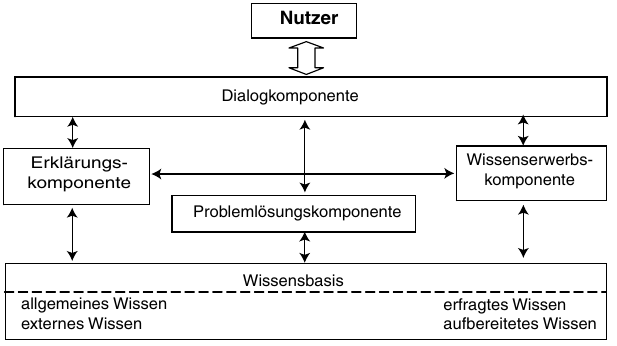
\includegraphics{bilder/aufbau_expertensysteme.png}}}
\caption{Aufbau eines Expertensystems.\label{fig:aufbau_expertensysteme}\protect\footnotemark}
\end{figure}
\footnotetext{\cite[S. 23]{laemmel}}

\newpage

\section{Problemlösung}
\label{sec:experten_systeme_problemloesung}
Um ein Problem zu lösen, wird typischerweise in den folgenden Schritten vorgegangen:
\begin{itemize}
    \item Charakterisierung der Problemdomäne
    \item Symbolische Repräsentation der Objekte
    \item Eingabe des Wissens in den Computer
    \item Stellen von Fragen
    \item Interpretieren der Antworten
\end{itemize}

Für die symbolische Repräsentation der Objekte ist es notwendig eine geeignete Sprache zu wählen. Dies können beispielsweise mathematische Relationen, Logik oder auch eine Programmiersprache sein. In der Informatik wird üblicherweise das Wissen über ein Problem direkt mittels Lösungsalgorithmen programmiert, bei der künstlichen Intelligenz jedoch, wird das Wissen getrennt von der Verarbeitungskomponente dargestellt. Dies hat den Vorteil, dass die Wissensbasis jederzeit ausgewechselt werden kann, die Verarbeitungskomponente jedoch bestehen bleibt. Ein Programm kann somit also für unterschiedliche Anwendungen verwendet werden. (vgl.~\cite[S. 28 - 30]{laemmel})

Eine Problemlösung geht immer von dem vorhandenen, expliziten Wissen --- z.B. in Form von Fakten --- aus. Aus dem expliziten Wissen kann implizites Wissen gewonnen, es können also Aussagen impliziert werden. Die Aufgabe der Verarbeitungskomponente ist es nun, das implizite Wissen abzuleiten. (vgl.~\cite[S. 30 - 31]{laemmel}) Dabei muss die Sprache zur Wissensrepräsentation sowie die Verarbeitungskomponente gewissen Kriterien genügen, Details siehe~\cite[S. 31]{laemmel}.

\section{Wissensarten}
\label{sec:experten_systeme_wissensarten}
Der Mensch nutzt mehrere Arten um Wissen abzubilden:
\begin{itemize}
    \item Relationales Wissen
    \item Vererbung von Eigenschaften
    \item Prozedurales Wissen
    \item Logisches Wissen
\end{itemize}
\label{itm:wissensarten}

\subsection{Relationales Wissen}
\label{subsec:relationales_wissen}
Relationales Wissen wiederspiegelt einfache Beziehungen zwischen Objekten. Ein Nachteil am relationalen Wissen ist, dass nur Fakten, aber keine logischen Abhängigkeiten abgebildet werden können.

\begin{lstlisting}[caption={Einfaches Beispiel von relationalem Wissen.}]
     Abenteuerreisen sind Reisen.
\end{lstlisting}

\newpage

\subsection{Vererbung von Eigenschaften}
\label{subsec:vererbung_eigenschaft}
Bei der Vererbung von Eigenschaften geht es darum, dass Eigenschaften einer Oberklasse an eine Unterklasse weitervererbt werden.

\begin{figure}[htbp]
\centering \rotatebox{0}{\scalebox{0.5}[0.5]{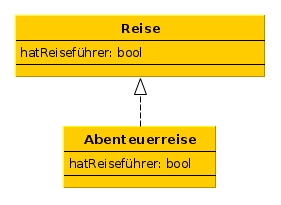
\includegraphics{bilder/experten_systeme_vererbung.png}}}
\caption{Einfaches Beispiel der Vererbung von Eigenschaften.\label{fig:experten_systeme_vererbung}\protect\footnotemark}
\end{figure}

\footnotetext{Eigene Darstellung mittels yEd.}

\noindent\rule[1ex]{\textwidth}{1pt}
\begin{wrapfigure}{l}{0.1\textwidth}
    \vspace{-14pt}
    
\includegraphics[width=0.1\textwidth]{bilder/owl.png}
\end{wrapfigure}
Eine Reise hat zum Beispiel einen Reiseführer. Definiert man nun, dass eine Abenteuerreise auch eine Reise ist (was für den Menschen bereits klar ist, da das Wort ja bereits Reise beinhaltet), ist es für den Menschen intuitiv klar, dass eine Abenteuerreise auch einen Reiseführer haben kann. Die Unterklasse Abenteuerreise erbt also die Eigenschaft der Möglichkeit eines Reiseführers von deren Oberklasse, der Reise.\\
\noindent\rule[1ex]{\textwidth}{1pt}

\subsection{Prozedurales Wissen}
\label{subsec:prozedurales_wissen}
Bei prozeduralem Wissen handelt es sich um Wissen, welches in bestimmten Situationen bestimmte Aktionen vorschreibt. Dies kann auch als Folge von Aktionen verstanden werden. So zum Beispiel das Aufschliessen einer Türe: Man steckt den (passenden) Schlüssel in da Schlüsselloch, dreht diesen, entsichert das Schloss, drückt die Türfalle nach unten und öffent schliesslich die Türe.

\begin{figure}[htbp]
\centering \rotatebox{0}{\scalebox{0.34}[0.34]{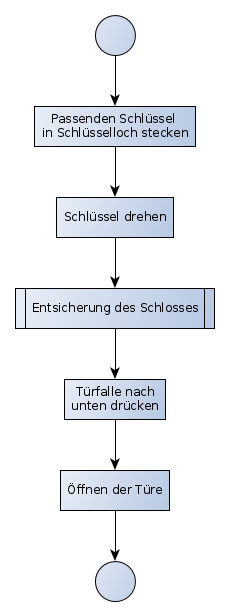
\includegraphics{bilder/experten_systeme_prozedurales_wissen.png}}}
\caption{Einfaches Beispiel von logischem Wissen.\label{fig:experten_systeme_prozedurales_wissen}\protect\footnotemark}
\end{figure}
\footnotetext{Eigene Darstellung mittels yEd.}

\newpage

\subsection{Logisches Wissen}
\label{subsec:logisches_wissen}

Bei logischem Wissen geht es im Grunde genommen um eine logische Implikation. Aus $A$ folgt $B$ bzw. $A \to B$, was so viel heisst wie ``Wenn $A$ gilt, kann geschlossen werden, dass auch $B$ gilt.''.

\noindent\rule[1ex]{\textwidth}{1pt}
\begin{wrapfigure}{l}{0.1\textwidth}
    \vspace{-14pt}
    
\includegraphics[width=0.1\textwidth]{bilder/owl.png}
\end{wrapfigure}
Möchte man zum Beispiel abbilden, dass ein Ausflug teambildend ist, so könnte man dies tun, indem man sagt, dass dieser für eine gewisse Anzahl Teilnehmer geeignet sein muss und/oder teambildende Eigenschaften hat. Oder, formal ausgedrückt: $A \vee B \rightarrow C$. Wobei $A$ die Tatsache darstellt, dass der Ausflug für eine gewisse Anzahl an Teilnehmern geeignet ist und $B$ die Tatsache, dass der Ausflug teambildend ist.\\
\noindent\rule[1ex]{\textwidth}{1pt}

\section{Wissensrepräsentationsformalismen}
\label{sec:wissensrepräsentationsformalismen}

Formalisiert man die unter~\ref{itm:wissensarten} genannten Arten des Wissens, so gelangt man zu den folgenden Wissenrepräsentationsformalismen:
\begin{itemize}
    \item Logik
        \begin{itemize}
            \item Aussagenlogik
            \item Prädkatenlogik erster Stufe
        \end{itemize}
    \item Semantische Netze und Frames
    \item Regelbasierte Sprachen
\end{itemize}

Wie unter~\ref{sec:experten_systeme_komponenten} beschrieben, bildet die Basis eines Expertensystemes unter Anderem eine Wissensdatenbank. Um solch eine Wissensdatenbank grafisch darzustellen und den Aufbau zu erleichtern, eignen sich Graphen besonders gut. Diese werden im nachfolgenden Kapitel ---~\ref{chap:graph_data}~\nameref{chap:graph_data} --- näher beschreiben.

\chapter{Graphrepräsentationen}
\label{chap:graph_data}

Sofern im Text nicht anders vermerkt, basiert das nachfolgende Kapitel auf~\cite{linkeddatatools}.

Graphen bilden eine der Grundlagen zur Darstellung von semantischen Daten, besonders für semantische Netze. In diesem Zusammenhang spricht man auch von Graphdatenbanken.

Der Unterschied gegenüber den gängigen Datenbanken, wie zum Beispiel den relationalen oder hierarchischen Datenbanken, liegt vorallem darin, dass Objekte beliebig verknüpft werden können.

Eine Graphdatenbank ist analog einem Graphen aufgebaut. Sie nutzt also dessen Struktur, bestehend aus Knoten, Kanten und Eigenschaften, um Daten bzw. Wissen darzustellen und abzulegen. Eine Graphdatenbank ist also ein Graph mit zyklenfreier Nachbarschaft. Dies bedeudet, dass jedes Element einen direkten Verweis auf seine benachbarten Elemente enthält und somit keine Abfragen auf dessen Relationen notwendig sind.

Die Knoten einer Graphdatenbank repräsentieren Entitäten. Eigenschaften sind auf Knoten bezogene Informationen. Kanten verbinden Knoten mit Knoten oder Knoten mit Eigenschaften und stellen die Beziehung zwischen diesen dar.

\begin{figure}[htbp]
\centering \rotatebox{0}{\scalebox{0.5}[0.5]{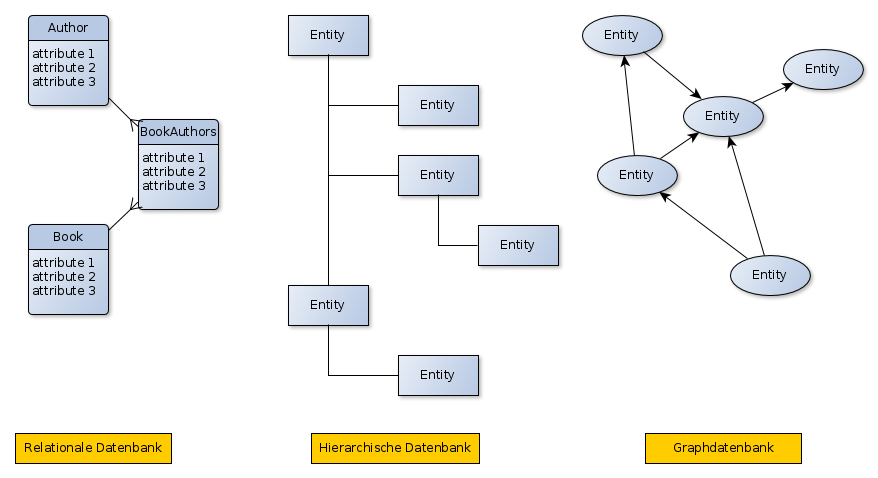
\includegraphics{bilder/datenbanktypen.png}}}
\caption{Darstellung der verschiedenen Datenbanktypen.\label{fig:datenbanktypen}\protect\footnotemark}
\end{figure}
\footnotetext{Eigene Darstellung mittels yEd, basierend auf~\cite{linkeddatatools}}

\newpage

Gegeben seien die folgenden Aussagen über Hotels:
\lstset{caption={Aussagen über Hotels},captionpos=b}
\begin{lstlisting}
    Ein Wellnesshotel ist ein Hotel.
    Ein Familienhotel ist ein Hotel.
    Wellnesshotels sind mit Familienhotels verwandt.
\end{lstlisting}

Verwendet man diese Hotelangaben um daraus eine Graphdatenbank zu erstellen, so ergibt sich folgende Graphdatenbank:
\begin{figure}[htbp]
\centering \rotatebox{0}{\scalebox{0.5}[0.5]{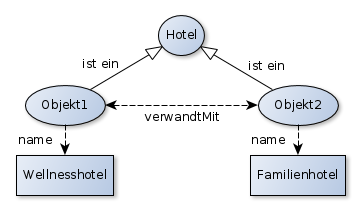
\includegraphics{bilder/hotels_graph.png}}}
\caption{Aussagen über Hotels als Graphdatenbank.\label{fig:hotels_graphdatenbank}\protect\footnotemark}
\end{figure}
\footnotetext{Eigene Darstellung mittels yEd}

In der Graphdatenbank existieren also zwei Objekte, \textit{``Objekt1''} und \textit{``Objekt2''}, mit den Eigenschaften \textit{``ist ein''}, \textit{``verwandtMit''} und \textit{``name''}.

\newpage

\noindent\rule[1ex]{\textwidth}{1pt}
\begin{wrapfigure}[6]{l}{0.1\textwidth}
    \vspace{-12pt}
    
\includegraphics[width=0.1\textwidth]{bilder/elephant.png}
\end{wrapfigure}
\label{elephant_graph_data}
Möchte man eine Graphdatenbank als Grundlage für eine semantische Datenbank aufbauen, so empfiehlt es sich, zuerst die wichtigsten Klassen und Individuen zu definieren. Es ist lohnend schon zu Beginn des Aufbaus schrittweise vorzugehen.

Nimmt man das Beispiel des Reiseplaners, ist es sinnvoll, nicht von Beginn an eine komplette Reise abzubilden, sondern zunächst mit der Abbildung lokaler Ausflüge zu beginnen. Später können diese mittels Logik zu einer Reise kombiniert werden.

Nach Überlegung ergeben sich die Klassen \textit{Ausflug}, \textit{Land}, \textit{Region} und \textit{Ort}. Doch wie gelangt man zu diesen Klassen? Nach unserer Erfahrung lohnt es sich, konkrete Fragen zu stellen, welche die semantische Datenbank schliesslich beantworten können sollte. Es ist zudem hilfreich, sich praktische Beispiele von der Anwendung solch einer Datenbank zu überlegen.

So könnte eine konkrete Anwendung eine Familie sein, welche einen eintägigen Ausflug planen möchte und deren Kinder bereits in einem Alter sind, in dem sie Beschäftigung benötigen. Dies führt schliesslich zu den Kriterien \textit{familienfreundlich}, \textit{regional} und \textit{actionreich}. Dies sind ausschliesslich Überlegungen für die spätere Entwicklung des Modelles. Eine Graphdatenbank kann nicht ohne Weiteres komplexe Anfragen im Sinne der genannten Kriterien oder Inhalte beantworten. Die Zusammenhänge könnte man durch Zuweisung von Kriterien an die Objekte statisch modellieren. Dies würde jedoch den Vorteil einer semantischen Datenbank zu Nichte machen, nämlich die Gewinnung von Schlüssen aus komplexen Zusammenhängen.

Hat man Klassen und Kriterien definiert, fällt auf, dass damit noch keine konkreten Anfragen beantwortet werden können. Es fehlen die Individuen und die Relationen.\\
Daher wird für einen Ausflug das Individuum \textit{``Seilpark Balmberg''} erstellt. Der Seilpark befindet sich in der Ortschaft \textit{Balmberg}, welche in der Region \textit{Solothurn} und damit in der \textit{Schweiz} liegt.\\
Damit erscheint es logisch, dass wenn ein Land in Regionen unterteilt ist, diese wiederum Orte beinhalten. Daher werden für Länder, Regionen und Orte ebenso Individuen erstellt.

Dies kann über die Relationen \textit{hatRegion} und \textit{hatOrt} abgebildet werden.

\begin{figure}[H]
\centering \rotatebox{0}{\scalebox{0.4}[0.4]{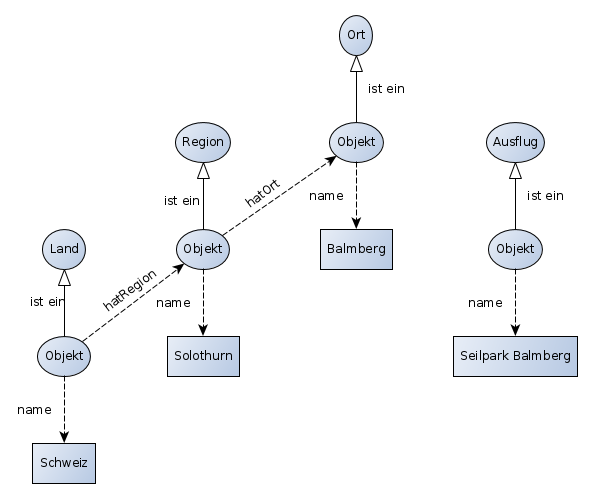
\includegraphics{bilder/graphen_beispiel_1.png}}}
\caption{Beispiel einer Graphdatenbank basierend auf dem Beispiel eines Reiseplaners\label{fig:protegebeispiel}\protect\footnotemark}
\end{figure}
\footnotetext{Eigene Darstellung mittels yEd\footnote{\url{http://www.yworks.com/en/products/yfiles/yed/}}}

Wie aus der Grafik ersichtlich ist, hat das Individuum \textit{Seilpark Balmberg} noch keine Relationen zu anderen Individuen. Daher ist zum jetzigen Zeitpunkt die Verknüpfung für Mehrwert bei Abfragen unklar.

\vspace{0.1pt}
\noindent\rule[1ex]{\textwidth}{1pt}

Da eine Graphdatenbank eine hohe Abstraktionsebene darstellt, werden Wissensrepräsentationsformen sowie ihre Anwendung im folgenden Kapitel genauer erläutert.

\chapter{Wissensrepräsentationsformen}
\label{chap:wissensrepFormen}

Nachdem wir im letzten Kapitel etwas über die Grundlage der Graphen sowie Graphdatenbanken erfahren haben, möchten wir hier auf konkrete Repräsentationsformen von Wissen eingehen.
In der Wissensmodellierung ( Knowledge Engineering) gibt es verschieden Wissensrepräsentationsformen um die Wissen in wissensbasierten Systemen formal abzubilden. Die so gesammelten Informationen werden als Wissensbank respektive Wissensbasis bezeichnet.~\cite{wikiWissensrep}

Das folgende Kapitel basiert auf dem Buch Künstliche Intelligenz\cite{laemmel}, es beschreibt einige der klassischen Wissensrepräsentationsformen.

Semantische Netze, Wissensnetze und Frames gehören zu den üblichen Wissensrepräsentationsformen. Dabei stehen die konkreten Objekte im Vordergrund. Und nicht, wie zum Beispiel bei Regeln, die Zusammenhänge und die logischen Abhängigkeiten.\\

Semantische Netze und Frames versuchen das menschliche Gedächtnis in adäquater Form abzubilden. Ursprünglich wurden Sie vor allem zur Analyse von Wörtern und Sätzen verwendend. Ein weiterer Punkt ist die einfach verständliche Darstellung von Klassen und deren Beziehungen. Des Weiteren haben die Konzepte der semantischen Netze und Frames die Entwicklung der objektorientierten Programmierung beeinflusst.

\section{Semantische Netze}
\label{sec:wissensrepFormen_semantischeNetze}

Eine zusammengehörige Gruppe von Objekten wird als Klasse bezeichnend. Ein einzelnes Objekt nennt sich auch Individuum. Zwischen den Objekten untereinander oder zu Klassen, oder zwischen Klassen untereinander gibt es Beziehungen. Es kann zwischen folgenden Beziehungen unterschieden werden:\\


"`ist eine"' Relation: \\
\noindent\hspace*{15mm} Es handelt sich also um Ober und Unterklassen.\\ 
\noindent\hspace*{15mm} Beispiel: Ein Baum ist eine Pflanze.\\

"`Instanz von"' Relation:\\
\noindent\hspace*{15mm} Die Relation beschreibt die Beziehung einer konkreten Instanz zu ihrer Klasse.\\
\noindent\hspace*{15mm} Beispiel: Birke ist eine Instanz der Klasse Baum\\

Eigenschaft:\\
\noindent\hspace*{15mm} Klassen und Objekte haben Eigenschaften\\
\noindent\hspace*{15mm} Pflanzen erzeugen Sauerstoff\\


Eigenschaften sind transitiv: Ist also ein Hund ein Tier und ein Tier ein Lebewesen ist auch ein Hund ein Lebewesen. Ausserdem halten sich Eigenschaften an das Gesetzt der Vererbung. Braucht also ein Tier Sauerstoff, braucht auch ein Hund Sauerstoff.

In Semantischen Netzen werden Objekte und Klassen als Knoten abgebildet. Beziehungen und Eigenschaften werden als Kanten dargestellt.
Einige Ausdrucksformen wie Existenzaussagen und Oder Aussagen können mit Semantischen Netzen nicht abgebildet werden. Obwohl sich aber nur zweistellige Beziehungen abbilden lassen sind komplexe Abbildungen wie zum Beispiel das modellieren einer Aktion möglich.

\section{Frames}
\label{sec:wissensrepFormen_frames}

In Frames werden die wesentlichen Charakteristika eines Objekts als Eigenschaften abgebildet und zusammengefasst. Dabei unterstützten Frames die Konzepte der Hierarchie und der Vererbung. Zudem können Frames auch generische Informationen wie Defaults, also Standartwerte und Wertebeschränkungen (Listen) enthalten.

\begin{figure}[htbp]
\centering \rotatebox{0}{\scalebox{0.5}[0.5]{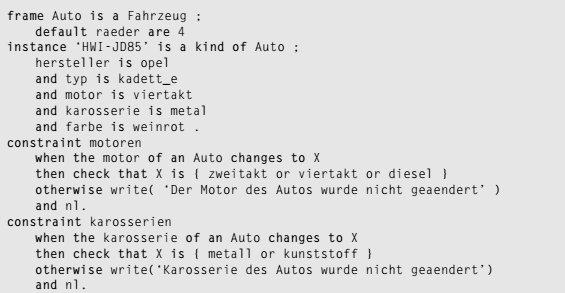
\includegraphics{bilder/framebsp.png}}}
\caption{Abbildung von Wissens mittels Frame.\label{fig:frames}\protect\footnotemark}
\end{figure}
\footnotetext{Beispiel aus KI BUCH - TODO ändern}

\section{Wissensnetze}
\label{sec:wissensrepFormen_Wissensnetze}
Bei Wissensnetzen handelt es sich um eine Art der Wissensrepräsentation, welche die Konzepte der semantischen Netzte verwenden. Dabei wird eine objektorientierte oder Frame-Darstellung des Wissens integriert. Zusätzlich erfolgt eine grafische Darstellung mittels Topic Maps. Diese wird auch Wissenslandkarte genannt. 

- Die Entfernung zweier Begriffe in der Wissenslandkarte bilden deren inhaltliche Nähe ab. Es werden also die semantischen Beziehung der Begriffe verwaltet. Dies ist eine grosse Unterstützt der Semantische Suche.

wie in den Semantischen Netzen werden Instanzen und Klassen in den Knoten abgebildet. Zusätzlich wird das Problem der Mehrfachvererbung umgangen indem das Konzept der Rollen eingeführt wird. Klassen werden so ausgebaut, das eine Instanz eine Bestimmte Rolle annehmen kann.
	
Wissensnetze haben sämtliche Voraussetzungen um effektives Wissensmanagement zu erreichen. Dafür muss das Wissen aber immer aktuell und entsprechen Umfangreich sein.\\
%\vspace{10pt}

%\newpage
\noindent\rule[1ex]{\textwidth}{1pt}
\vspace{0.1pt}
\begin{wrapfigure}{l}{0.1\textwidth}
    \vspace{-19pt}
    
\includegraphics[width=0.1\textwidth]{bilder/owl.png}
\end{wrapfigure}
Ein sehr wichtiger und Zeitintensiver Teil des Knowledge Engineering ist die tatsächliche Modellierung. Sich also zu überlegen ob eine abzubildende Information ein Objekt, eine Instanz oder eine Eigenschaft ist. Oder ob sie gar als Regel abgebildet werden kann. Dazu später mehr. Uns scheint an dieser Stelle aber wichtig zu erwähnen, dass uns das Semantischen Netz ein sehr gutes Hilfsmittel war, einen Überblick über die Informationen und ihre Verwendbarkeit zu erhalten.
An unserem konkreten Beispiel könnte dies folgendermassen aussehen: 

\begin{figure}[H]
\centering \rotatebox{0}{\scalebox{0.5}[0.5]{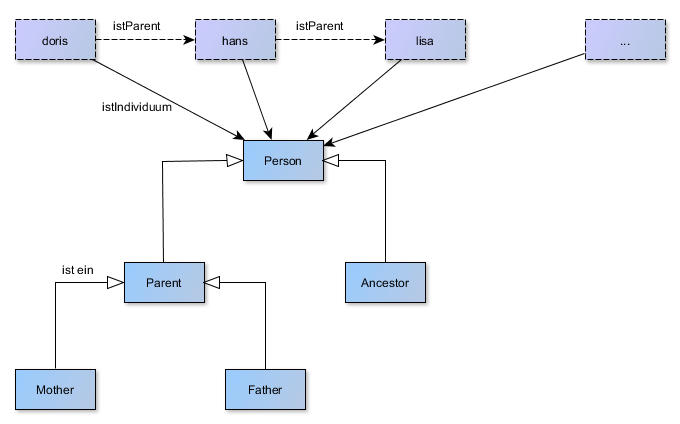
\includegraphics{bilder/familyEinfachesNezt.png}}}
\caption{Abbildung von Wissens mittels Semantischen Netzen.\label{fig:semantischesNetz}\protect\footnotemark}
\end{figure}
\footnotetext{Eigene Darstellung mittels yEd}

Dies sieht hier ja alles ziemlich simpel aus. Wie aber bereits oben erwähnt, handelt es sich um einen Übersicht der Informationen. Würde man das Wissen direkt so in die Semantische Datenbank übertragen, wäre diese nicht viel mächtiger als eine traditionelle Wissensspeicherung. Dies führen wir zu einem späteren Zeitpunkt noch genauer aus.\\

\vspace{0.1pt}
\noindent\rule[1ex]{\textwidth}{1pt}


% Einträge im Verzeichnis erscheinen lassen ohne hier eine Referenz einzufügen
%\nocite{kopka:band1}

\chapter{Wissen abbilden mittels Ontologien}
\label{chap:ontologien}

Die bisherigen Kapitel bieten einen groben Überblick über Objekte und deren Anwendung. Um bei der Wissensmodellierung von Nutzen zu sein, müssen sie aber in eine geeignete Form gebracht werden.\\
Wissen wird im Knowledge-Engineering zum Beispiel in Form von Ontologien abgelegt.

Der Begriff Ontologie wird in verschiedenen wissenschaftlichen Bereichen verwendet, so zum Beispiel in der Philosophie, der Psychologie und der Informatik. In diesem Dokument soll nur der Aspekt der Informatik erklärt werden.

Sofern nicht anders vermerkt, basiert das folgende Kapitel auf~\cite{IspekOntoBedeutung} sowie~\cite{ISpekOntoGeschichte}.

In der Informatik steht Ontologie für ``\ldots eine formale Beschreibung des Wissens in einer Domäne in der Form von Konzepten der Domäne, deren Beziehung untereinander und der Eigenschaft dieser Konzepte und Beziehungen, sowie der in der Domäne gültigen Axiome und Prinzipien.''~\cite[S. 310]{ISpekOntoGeschichte}.

Zum besseren Verständnis wird diese Definition im folgenden Abschnitt kurz untersucht:
\begin{itemize}
    \item \textit{Domäne}

        Unter einer Domäne versteht man einen Ausschnitt der Welt, dessen Grenzen klar definiert sind. Die Domäne und ihre Grenzen werden durch den Anwendungsfall festgelegt.

    \item \textit{Konzepte}

        Konzepte werden in anderen Teilen dieses Dokumentes als Objekte oder Klassen bezeichnet. Dabei kann es sich um materielle Konzepte, wie zum Beispiel Teile eines Wagens oder um immaterielle Konzepte, wie zum Beispiel die Lösungssuche, handeln.

    \item \textit{Beziehungen}

        Objekte stehen in Beziehungen zueinander. Es werden die Beziehungen ``ist ein'' und ``Instanz von'' unterschieden. In unserem Beispiel sind eine Abenteuerreise eine Reise und der Seilpark Balmberg eine Instanz eines Ausfluges ($Abenteuerreise\;istEin\;Ausflug$ und $SeilparkBalmberg\;instanzVon\;Ausflug$).\\
        Die Eigenschaften eines Objektes werden auch als Beziehungen dargestellt (eine Reise hat einen Reiseführer).

    \item \textit{Axiome und Prinzipien}

        Damit werden die in der Domäne vorhandenen Regeln bezeichnet.
\end{itemize}

Mit diesen Elementen sind alle wichtigen Punkte einer Ontologie abgedeckt. Dabei ist es, wie in der Definition festgelegt, wichtig, dass die gesamte Abbildung in einer formalen Sprache beschrieben wird.

\section{Anwendung von Ontologien}
\label{sec:ontologien_onto_anwendung}
Ontologien werden für wissensbasierte Anwendungen verwendet. Konkret werden sie hauptsächlich dort verwendet, wo Semantik zur Formulierung von Informationen genutzt wird. Eines der bekanntesten Beispiele ist das semantische Web. Im Gegensatz zum syntaktischen Web versucht das semantische Web Zeichen nicht nur abzugleichen, sondern auch ein Verständnis und Schlussfolgerungen einzubauen.

Die Aufgabe von Ontologien ist die Ermöglichung und Verbesserung von Kommunikation zwischen Computeranwendungen untereinander und zwischen Computeranwendungen und Mensch. Wichtig: Es darf sich immer nur um eine bestimmte Wissensdomäne (Domain Ontology) handeln. Diese muss klar abgegrenzt sein. \\
Einige Berufsgruppen haben bereits begonnen, ihr Wissen mit Hilfe von standardisierten Sprachen abzubilden. Diese Sprachen, wie die in Kapitel~\ref{chap:owl} vorgestellte Sprache OWL, wurden vom W3C-Konsortium (World Wide Web Consortium) standardisiert.

\subsection{Anwendung des semantischen Webs}
\label{subsec:ontologien_onto_SemantikWebAnwendung}
Eine Anwendung des semantische Webs führt zu der Gewinnung von zusätzlichem Wissen. Dies geschieht durch eine Wissensbasis in Form einer Wissensdatenbank und einer Inferenzmaschine. Ein Ontologieschema legt in der Wissensbasis fest, welche Arten von Aussagen möglich sind. Die Aussagen enthalten das konkrete Wissen. Sowohl das Schema, wie auch die Wissensabbildung werden in einer formalen Sprache, wie z.B. OWL oder RDFS, abgebildet.

\begin{lstlisting}[caption={Beispiel einer Aussage in einer Wissensbasis.}]
Eine Abenteuerreise ist eine Reise.
\end{lstlisting}

In der einfachsten Anwendung kann das abgelegte Wissen direkt abgefragt werden. Bei komplexeren Anfragen sind die Funktionalitäten einer \textit{Inferenzmaschine} notwendig. Mittels Inferenzregeln ist diese fähig Schlussfolgerungen zu ziehen und dadurch neue, komplexe Aussagen zu generieren.

Die Transitivitätsregel ist eine einfache, von der Inferenzmaschine verwendete Regel: ``Wird eine Relation $p$ als transitiv deklariert und es gilt $x p y$ und $y p z$, dann kann $x p z$ gefolgert werden.''~\cite[S. 289]{IspekOntoBedeutung}
Dem Entwickler ist es möglich, neben den vorhandenen Regeln, wissensdomänenspezifische Regeln zu spezifizieren. Die Inferenzmaschine berücksichtigt diese bei ihrer Auswertung.

\begin{lstlisting}[caption={Beispiel einer Regel in einer Wissensbasis.}]
Handelt es sich bei einem Objekt um eine Reise, benötigt das Objekt mindestens vier Teilnehmer/innen und ist das Objekt teambildend, so handelt es sich bei dem Objekt auch um einen Teamevent.
\end{lstlisting}

Damit eine Inferenzmaschine Schlüsse ziehen kann, muss die Wissensbasis in einer formalen Sprache vorliegen. Sie darf keine syntaktischen Fehler enthalten. Das Schema und die Aussagen werden von der Maschine geladen und intern als Graph gespeichert (siehe Kapitel~\ref{chap:wissensrepFormen}).\\
Durch einen Algorithmus zum Abgleich von Graphen werden Abfragen implementiert. Durch wiederholtes Anwenden von Regeln können \textit{Schlussfolgerungen} gezogen werden.\\ Die Anwendung dieser Regeln erfolgt wiederum mit Hilfe von Algorithmen zum Abgleich von Graphen. Die dadurch entstandenen Aussagen werden der Wissensbasis hinzugefügt und stehen für Abfragen zur Verfügung.

\noindent\rule[1ex]{\textwidth}{1pt}
\begin{wrapfigure}[8]{l}{0.1\textwidth}
    \vspace{-14pt}
    
\includegraphics[width=0.1\textwidth]{bilder/owl.png}
\end{wrapfigure}
Wir brauchen Ontologien. Dabei spielt die Wahl der Domäne eine grosse Rolle. Bei unserer Wissensmodellierung haben wir gelernt, das sich nicht jeder Themenbereich als Domäne eignet.
Bei Umsetzung der ursprünglichen Problemdomäne, nämlich dem Erlernen des Programmierens anhand der Programmiersprache Prolog, mussten wir feststellen, dass diese nicht als Domäne geeignet ist. Zum Beispiel lässt sich das Konzept der Rekursion in einer Ontologie zwar lexikalisch abbilden, der Mehrwert (einer Ontolgie gegenüber der herkömmlichen Wissensabbildung) in Form von Inferenz, ist jedoch nicht gegeben. Die Möglichkeiten einer Wissensmodellierung anhand einer Ontologie sind bei Themen, die Inferenz und damit Schlussfolgerungen zulassen, viel grösser.
\noindent\rule[1ex]{\textwidth}{1pt}

Im nachfolgenden Kapitel wird eine Erklärung gegeben, wie Inferenz und Resolution zum Ziehen von Schlüssen verwendet werden.

\chapter{Inferenz und Resolution}
\label{chap:inferenz_resolution}

\section{Inferenz}
\label{sec:inferenz}
Grundsätzlich geht es bei Inferenz um den Prozess von Schlussfolgerungen mithilfe von Resolution (siehe~\ref{sec:resolution}). Die logische Inferenz ist ein Prozess der Inferenz und Resolution, welcher die Folgebeziehungen zwischen Sätzen zum Ausdruck bringt.~\cite[S. 163]{russel}.

\subsection{Inferenz in Computern}
\label{subsec:inferenz-in-computer}

Das grundsätzliche Problem bei Computern im Bezug auf Inferenz ist, dass ein Computer keine Interpretation vornehmen kann und nichts über die (Um-) Welt weiss, bzw.\ nur, was in seiner Wissensdatenbank gespeichert ist (vgl.~\citet[S. 164]{russel}).


Angenommen, man möchte einen Computer fragen

\lstset{caption={Beispielanfrage an eine Wissensdatenbank eines Computers},captionpos=b}
\begin{lstlisting}
    ``Ist eine Abenteuerreise eine Reise?''
\end{lstlisting}

so weiss der Computer weder was ein Abenteuerreise ist, noch kennt er das Konzept des Reisens an sich. Das Einzige, was er tun kann, ist, in der Wissensdatenbank nach 

\lstset{caption={Aussage in einer Wissensdatenbank eines Computers},captionpos=b}
\begin{lstlisting}
    ``Eine Abenteuerreise ist eine Reise.''
\end{lstlisting}

zu suchen. Findet der Computer diese Aussage in der Wissensdatenbank, so spielt es keine Rolle, dass er das Konzept der Abenteuerreise oder des Reisens nicht kennt. Die Schlussfolgerung, dass eine Abenteuerreise eine Reise ist, trifft unter allen Gegebenheiten und Interpretationen zu, welche für die Wissensdatenbank zutreffen (vgl.~\cite[S.164]{russel}).

Zusammengefasst kann gesagt werden, dass die formale Inferenz in der Lage ist, gültige Schlussfolgerungen zu ziehen, auch wenn der Computer die Interpretationen des Anwenders nicht kennt. Der Computer zieht immer logisch gültige Schlüsse, unabhängig von der (menschlichen) Interpretation. Da der Mensch in der Regel die Interpretation kennt, erscheinen die Schlüsse dem Menschen logisch (vgl.~\cite[S. 165]{russel}).

\section{Resolution}
\label{sec:resolution}

Resolution, aus dem Lateinischen ``resolutio'', zu Deutsch ``Auflösung'', ist eine Verallgemeinerung des Modus Ponens~\cite[S. 279]{russel}. Die Methode der Resolution wurde 1965 von J. A. Robinson entwickelt, dabei handelt es sich um einen vollständigen Algorithmus der Theorembeweisung für Prädikatenlogik erster Stufe.~\cite[S. 18]{russel} In der einfachsten Form handelt es sich bei der Resolution um eine Inferenz-Regel der Aussagenlogik.~\cite[S. 277]{russel}

Eine Verallgemeinerung der einfachen Form der Inferenz-Regel zur Resolution kann als Regel zur kompletten Inferenz der Prädikatenlogik erster Stufe genutzt werden.~\cite[S. 278]{russel}

\section{Inferenz und Resolution zum Ziehen von Schlüssen}
\label{sec:inferenz_praktisch}
Inferenz in der Semantik kann grundsätzlich als das Entdecken von neuen Beziehungen zwischen Entitäten beschrieben werden. Dies heisst, dass automatische Prozeduren, in Form von so genannten \textit{Reasonern}, neue Beziehungen ableiten. Wie die neuen Beziehungen generiert werden ist eine Frage der Implementation, so z.B. durch Hinzufügen zu den Daten oder durch eine einfache Rückgabe dieser (vgl.~\cite[Abschnitt 1]{w3inference}).

Reasoner sind Komponenten, welche eine Folgerung von implizitem Wissen zulassen bzw.\ bieten. Es handelt sich um eine Art ``Verstehen'' durch Maschinen. Ziel ist es implizites Wissens aus explizitem Wissen, in Form einer Ontologie, zu erschliessen.

Eine detaillierte Beschreibung solch einer praktischen Umsetzung, in Form des \textit{Pellet}-Reasoners der Firma Clark \& Parsia, findet sich im~\autoref{sec:inferenz_pellet}. Dieser basiert auf Beschreibungslogik.  Eine Einführung der Grundlagen der Beschreibungslogik folgt im nächsten Abschnitt.

\subsection{Beschreibungslogik}
\label{subsubsection:beschreibungslogik}
Beschreibungslogiken sind Formalismen um Wissen darzustellen, dabei sind sie eine Teilmenge der Prädikatenlogik. Sie stellen den Kern von Wissensrepräsentationssystemen dar, in dem sie eine Struktur für eine Wissensbasis und den damit verbundenen Methoden zur Folgerung bieten (vgl.~\cite{dl:baader2003}).

Die Struktur, welche Beschreibungslogiken als Wissensbasis bereitstellen, besteht aus einem Schema (Tbox, Regeln), sowie aus den Daten (Abox, Fakten).

Details zu Beschreibungslogiken finden sich unter~\cite{dl:baader2003}.

\subsubsection{Interpretation}
\label{subsubsection:beschreibungslogik_Interpretation}
``Man bezeichnet die Zuordnung von Ereignissen aus einer realen Welt zu aussagenlogischen Variablen als Interpretation.''~\cite[S. 36]{laemmel}

\begin{lstlisting}[caption={Definition einer Interpretation \protect\footnotemark}]
    Sei M die Menge aller aussagenlogischen Formeln. Eine Funktion
        $I : M \rightarrow \{ W , F \}$
    heisst Interpretation.
\end{lstlisting}
\footnotetext{\cite[S. 36]{laemmel}}

\subsubsection{Modell}
\label{subsubsection:beschreibungslogik_modell}
\begin{lstlisting}[caption={Definition Modell \protect\footnotemark}]
    Sei $I$ eine Interpretation und $X$ eine aussagenlogische Formel.
    Ist $X$ unter $I$ wahr, so bezeichnet man $I$ als Modell von $X$.
\end{lstlisting}
\footnotetext{\cite[S. 37]{laemmel}}

\subsubsection{Semantische Folgerung}
\label{subsubsection:beschreibungslogik_semfol}
``Der Zusammenhang von Formeln kann durch den Begriff der semantischen Folgerung dargestellt werden.''~\cite[S. 39]{laemmel}

\begin{lstlisting}[caption={Definition semantische Folgerung\protect\footnotemark}]
    Sei $X$ eine Menge von aussagenlogischen Formeln, $Y$ eine aussagenlogische Formel.
        $Y$ ist eine semantische Folgerung von $X$
    falls jedes Modell von $X$ auch Modell von $Y$ ist.
    Man schreibt dafür $X \models Y$ und sagt auch $Y$ folgt aus $X$.
\end{lstlisting}
\footnotetext{\cite[S. 39]{laemmel}}

\subsubsection{Ableitbarkeit}
\label{subsubsection:beschreibungslogik_ableitbarkeit}
Es ist erforderlich, ``\dots dass das Folgern von Formeln auf der Ebene der Gültigkeit von der Berechnung von Formeln auf der Inferenzebene unterschieden wird. Dies wird mit dem Begriff des Ableitens getan.''~\cite[S. 42]{laemmel}

\begin{lstlisting}[caption={Definition Ableitbarkeit\protect\footnotemark}]
    $Y$ ist aus $X$ ableitbar,
        $X \vdash Y$
    wenn eine endliche Folge von Inferenzschritten existiert,
    so dass man von $X$ zu $Y$ gelangt.
\end{lstlisting}
\footnotetext{\cite[S. 42]{laemmel}}

\subsubsection{Korrektheit und Vollständigkeit}
\label{subsubsection:beschreibungslogik_vollstanendigkeit}
``Der Bezug zwischen beiden Begriffen (semantische Folgerung und Ableitbarkeit, Anm.\ der Autoren) wird durch die Begriffe der Korrektheit und der Vollständigkeit hergestellt.''~\cite[S. 43]{laemmel}

\begin{lstlisting}[caption={Definition Korrektheit und Vollständigkeit\protect\footnotemark}]
    Ein Beweis-Verfahren heisst korrekt, wenn für beliebige Formeln $X, Y$ gilt:
        Falls $X \vdash Y$ gilt, dann gilt auch $X \models Y$.
    Ein Beweis-Verfahren heißt vollständig, wenn für beliebige Formeln $X, Y$ gilt:
        Falls $X \models Y$ gilt, dann gilt auch $X \vdash Y$.
\end{lstlisting}
\footnotetext{\cite[S. 43]{laemmel}}

\section{Pellet}
\label{sec:inferenz_pellet}
Sofern im Text nicht anders vermerkt, basiert das nachfolgende Kapitel auf~\cite{sirin:pellet05}.

Bei Pellet handelt es sich um einen Reasoner auf Basis von Beschreibungslogik. Eine syntaktische Variante von Beschreibungslogik ist OWL.\@ Pellet wurde von Grund auf für die OWL-DL~\footnote{\url{http://www.w3.org/TR/owl-ref/\#OWLDL}} Sprache entwickelt. Diese ist wiederum eine Teilsprache von OWL-full, siehe~\autoref{chap:owl}.

Eine komplette Unterstützung des OWL-full Profils ist so nicht möglich, da dieses nicht entscheidbar ist, daher beschränkt sich Pellet auf die Verwendung von OWL-DL\@.~\cite[Seite 13]{sirin:pellet05}

\begin{figure}[htbp]
\centering \rotatebox{0}{\scalebox{0.5}[0.5]{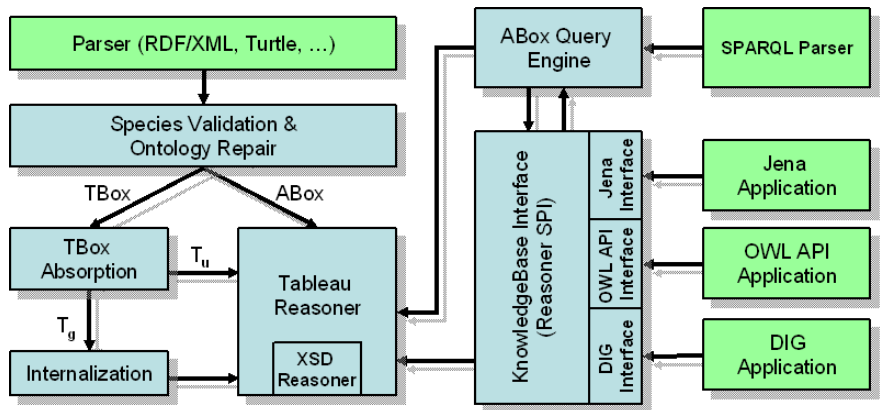
\includegraphics{bilder/pellet_komponenten.png}}}
\caption{Hauptkomponenten des Pellet-Reasoners.\label{fig:pellet_komponenten}\protect\footnotemark}
\end{figure}
\footnotetext{\cite[S. 6]{sirin:pellet05}}

Die obenstehende Abbildung zeigt die Hauptkomponenten von Pellet. Dabei ist der Tableaux-Reasoner die Kernkomponente des Systems, welche die Wissensbasis auf deren Konsistenz prüft. Der Designentscheid, dass Pellet von Anfang an für OWL entwickelt wurde, führte zu einer modularen Struktur. Module sind z.B.\ ein Reasoner zur Datentypenprüfung eines XML-Schemas oder eine ``Query-Engine''. Genaueres dazu wird in den nachfolgenden Abschnitten beschrieben.

Hier eine Übersicht der wichtigsten Komponenten von Pellet:
\begin{table}[H]
\centering
\fbox{\begin{minipage}[t]{0.48\linewidth}%
    \begin{tabbing}
        Abkürzung \= Bezeichnung ******** \= Beschreibung \kill \\
        ---           \> Tableaux-Reasoner  \> Komponente, zum Ziehen von Schlüssen durch Konsistenzprüfung \\
                      \>                    \> einer Ontolgie.  \\
        \textbf{Abox} \> Assertional Box    \> Komponente, welche Aussagen zu Individuen enthält, \\
                      \>                    \> also OWL-Fakten wie Typen, Eigenschaftswerte und logische Äquivalenz. \\
        \textbf{Tbox} \> Terminological Box \> Komponente, welche Klassenaxiome enthält, also OWL-Axiome \\
                      \>                    \> wie z.B. Unterklassen, Gleichheit von Klassen und Klasseneinschränkungen. \\
        \textbf{KB}   \> Knowledge Base     \> Eine Kombination einer Abox und Tbox, daher eine komplette OWL-Ontologie.
    \end{tabbing}
\end{minipage}}\hfill
\captionof{table}{Beschreibung der wichtigsten Komponenten von Pellet\protect\footnotemark}
\footnotetext{\cite[S. 4]{sirin:pellet04}}
\end{table}


\subsection{Vorgehen des Pellet-Reasoners}
\label{subsection:inferenz_pellet_vorgehen}
Wird eine Ontologie mittels Parser geladen, wird diese auf deren Gültigkeit bezüglich OWL-DL geprüft. Während des Ladens werden Klassenaxiome in der Tbox, Aussagen über Individuen in der Abox abgelegt. Die Axiome der Tbox werden durch das Standardverfahren von OWL-DL-Reasonern vorverarbeitet. Sie werden durch verschiedene Optimierungsverfahren vereinfacht (siehe \ref{subsection:inferenz_pellet_opti)} und anschliessend in den Tableaux-Reasoner eingespiesen.

\subsubsection{Laden und Parsen der Daten}
\label{ssubsection:inferenz_pellet_parsing}
Pellet bietet diverse Schnittstellen um Ontologien zu laden. Pellet selbst implementiert keinen RDF/OWL-Parser, ist aber in verschiedenen RDF/OWL-Werkzeugen, welche solch einen Parser anbieten, integriert. Dabei unterstützt Pellet die unterschiedlichen Datenstrukturen der Werkzeuge. Weiter stellt der Reasoner Schnittstellen um Anfragen der Werkzeuge zu beantworten zur Verfügung.

\subsubsection{Tableaux-Reasoner}
\label{ssubsection:inferenz_pellet_tableaux}
Der Tableaux-Reasoner hat nur eine Funktion: Eine Ontologie auf ihre Konsistenz zu prüfen. Eine Ontologie ist genau dann konsistent, wenn eine Interpretation der Ontologie existiert, welche alle Fakten und Axiome dieser erfüllt.~\cite{w3owlsemantics} Solch eine Interpretation wird als Modell der Ontologie bezeichnet.

Der Tableaux-Reasoner sucht nach solch einem Modell durch Vervollständigung. Dieses wird inkrementell als eine Art Tafel (eben, Tableau) aufgebaut. Die Vervollständigung beginnt mit einem initialen Graphen der Abox. Dabei repräsentieren die Knoten Individuen und Literale (z.B. Zeichenketten, Datumswerte oder auch Nummern). Jedem Knoten wird der entsprechende (Daten-) Typ zugewiesen. Die gerichteten Kanten zwischen den Knoten, stellen die Eigenschaften dar. %mira ab hier
Dem initialen Graphen wird die Negation der Folgerung hinzugefügt.


Durch wiederholtes Anwenden der Regeln zur Erweiterung des Graphen, versucht der Reasoner einen widerspruchsfreien Graphen zu bilden. Dies tut er solange bis entweder ein Widerspruch (Kontradiktion) auftritt oder keine Regeln mehr anwendbar sind.

Der Tableaux Algorithmus basiert auf dem Tableau Kalkül. Dabei soll ein mittels Wiederspruchsbeweis aufgezeigt werden, das eine Interpretation existiert in der sowohl sämtliche Prämissen (Anforderungen) als auch die Negation der Konklusion (Folgerung) wahr ist. Kann ein solches Modell aufgezeigt werden, kann beweisen werden das die Ursprüngliche "`Formel"' falsch ist. Die in der ABox definierten Daten sind also dann Konsistenz wenn beim Aufbau des Baums inklusive der Negation ein Widerspruch auftritt.~\cite{baumkalkül}

Für das Tableau Kalkül werden Transformationsregeln benötigt. Mit diesen Regeln wird ein Argument unter einer Interpretation wahr gemacht. Es wird also ein Modell erzeugt.\cite{baumkalkül}

Nachfolgend sind die Transformationsregeln zum erzeugen von Modellen aufgelistet.

\begin{table}[H]
\centering
\fbox{\begin{minipage}[t]{0.48\linewidth}%
    \begin{tabbing}
        Argument \= Modell ******** \= Beschreibung \kill \\
        P           \> I(P) = W  \> \\
        $\lnot$ Q       \>    I(Q) =F          \>   \\
        P $\lang$ Q \> I(P) = I(Q) = W    \>  \\
        P $\lor$ Q 	\>	I(Q) = W    \> oder  \\	
									\>	I(P) = W    \> oder  \\		
									\>	beides    	\>   			\\		
        P $\rightarrow$ Q 	\>	I(P) = W    \> oder  \\	
									\>	I(Q) = F    \> oder  \\		
									\>	beides    	\>   			\\																								
    \end{tabbing}
\end{minipage}}\hfill
\captionof{table}{Transformationsregeln \protect\footnotemark}
\footnotetext{\cite{baumkalkül}}
\end{table}

Das Tableaukalkül läuft folgendermassen ab:
%Der generelle Prozess (der Folgerung TODO: wieso der Folgerung??)  läuft wie folgt ab:
\begin{itemize}
    \item Umwandlung eines Konzeptes bzw.\ der Konzepte in die negierte Normalform (NNF) ( die Negation $ \neg $ befindet sich vor Konzeptnamen.)
    \item Ablegen des umgewandelten Konzeptes als $ C_0 $.
        Der Algorithmus hat also die Datenbasis (Abox) $ A_0 = {C_0(x_0)} $
    \item Regeln zur Transformation auf die Datenbasis (Abox) so weit als möglich anwenden.
    \item Wurde eine gültige Datenbasis (Abox) gefunden, so ist $ C_0 $ erfüllbar. (TODO: also wenn beim anwenden der Transformationsregeln auff die NNF ein Widerspruch Auftritt)
    \item Wurde keine gültige Datenbasis unter Berücksichtigung aller (Such-) Pfade gefunden, so ist $ C_0 $ nicht erfüllbar.
\end{itemize} (vgl.~\cite{horrocks2002} und~\cite{horrocks2005})



Mit dem folgenden Beispiel soll veranschaulicht werden wie das Tableaukalkül im Reasoner angewendet wird:

TODO: Dieses Beispiel habe ich im Moment auf Papier vorbereitet. Bevor ich das hier mit viel Aufwand in s Latex bastle können wirs ja mal zusammen anschauen. Ich habs aber glaub. Ich mach aber morgen noch weiter. Den Teil unter TODO überleg ich mir noch, wie ich den einarbeite. aber ich hab da schon neh idee... :D

% TODO ----------------------------

%Nachfolgend ein Beispiel, gegeben sei:
%$ Prolog \subseteq LogischeProgrammiersprache, LogischeProgrammiersprache \subseteq Programmiersprache $
%Man stellt nun folgende Anfrage:
%$ if Prolog \subseteq Programmiersprache $
%
%Der Prozess der Folgerung findet nun wie folgt statt:
%\begin{itemize}
    %\item Testen, ob ein Individuum existiert, welches eine logische Programmiersprache, aber keine Programmiersprache ist.\\
        %Man möchte also die Erfüllbarkeit des Konzeptes $ C_0 = (Prolog \sqcap \neg Programmiersprache) $ testen.\\
        %Es wird also versucht die Erfüllbarkeit mittels Widerspruch zu beweisen.
    %\item $ C_0(x) \Rightarrow Prolog(x), (\neg Programmiersprache)(x) $
    %\item $ Prolog(x) \Rightarrow LogischeProgrammiersprache(x) $
    %\item $ LogischeProgrammiersprache(x) \Rightarrow Programmiersprache(x) $
        %$ \Rightarrow $ Konflikt!
%\end{itemize}
%Wie ersichtlich ist, ist das Konzept $ C_0 $ nicht erfüllbar, die Anfrage $ Prolog \subseteq Programmiersprache $ trifft somit innerhalb der gegebenen Ontologie zu.
%
%Alle anderen Aufgaben zum Ziehen von Schlüssen können als Konsistenzprüfungen definiert werden.
%
%Die Strategien zur Vervollständigung eines Modelles werden unter~\cite[Seiten 7 bis 9]{sirin:pellet05} ausführlich beschrieben.
%
%
%
%
%
%Der generelle Prozess der Folgerung läuft wie folgt ab:
%\begin{itemize}
    %\item Umwandlung eines Konzeptes bzw.\ der Konzepte in die negierte Normalform (NNF), die Negation $ \neg $ befindet sich vor Konzeptnamen.
    %\item Ablegen des umgewandelten Konzeptes als $ C_0 $.
%
        %Der Algorithmus hat also die Datenbasis (Abox) $ A_0 = {C_0(x_0)} $
    %\item Regeln zur Transformation auf die Datenbasis (Abox) so weit als möglich anwenden.
    %\item Wurde eine gültige Datenbasis (Abox) gefunden, so ist $ C_0 $ erfüllbar.
    %\item Wurde keine gültige Datenbasis unter Berücksichtigung aller (Such-) Pfade gefunden, so ist $ C_0 $ nicht erfüllbar.
%\end{itemize} (vgl.~\cite{horrocks2002} und~\cite{horrocks2005})
%
%Gegeben seien folgende Datensätze, welche Regeln definieren
%
%\begin{lstlisting}[caption={Aussagentripel bestehend aus Objekt, Prädikat und Subjekt},captionpos=b,label=lst:reasoning_seilpark]
    %``Schweiz hatRegion Solothurn.''
    %``Solothurn hatOrt Balmberg.''
    %``Seilpark istUnterklasseVon Ausflug.''
    %``Seilpark hatStandort Balmberg.''
%\end{lstlisting}

%definiert.
%
%Unterstützt nun ein Programm Inferenz, z.B. durch einen Reasoner, so kann dieser schlussfolgern, dass der Ausflug \textit{Seilpark} in der Region Solothurn ist (vgl.~\cite[Abschnitt `Examples']{w3inference}).

% TODO END ----------------------------

\subsubsection{Datentypenprüfung}
\label{ssubsection:inferenz_pellet_datatypes}
In OWL werden Datentypen in einem XML-Schema beschrieben. Dadurch sind viele einfache Datentypen bereits gegeben, so z.B.\ numerische Datentypen (Ganz- und Fliesskommazahlen) und Zeichenketten. OWL bietet des Weiteren die Möglichkeit eigene Datentypen zu definieren.

Das Modul zur Datentypenprüfung prüft ob die Schnittmenge von Datentypen konsistent ist. Eine Schnittmenge von Datentypen ist dann inkonsistent, wenn diese keine Elemente gemeinsam haben.

Der Tableaux-Reasoner nutzt das Modul um für jeden Literal-Knoten des Graphen der Abox festzustellen, ob die Schnittmenge aller Datentypen eines jeden Knotens erfüllbar ist.

\subsubsection{Schnittstelle zur Wissensdatenbank (KB)}
\label{ssubsection:inferenz_pellet_kb}
Alle Aufgaben zum Ziehen von Schlüssen können auf eine Konsistenzprüfung anhand der Wissensdatenbank (KB) reduziert werden. Die Schnittstelle zur Wissensdatenbank entscheidet, wann die Konsistenz der Abox geprüften werden muss, wann alle Konzepte neu klassifizert werden müssen oder wann alle Individuen umgesetzt werden. %TODO WTF!?

Die Schnittstelle bietet die Möglichkeit beliebige atomare Anfragen zu beantworten. Diese können Klassen, Eigenschaften oder Individuen betreffen. Wahrheitsabfragen werden in Erfüllbarkeitsprobleme umgewandelt.

Für Anfragen, welche mehrere Ergebnisse zurückliefern, sind theoretisch mehrere Konsistenzprüfungen notwendig. Da dies aber sehr aufwändig ist, werden die im~\autoref{subsection:inferenz_pellet_opti} beschriebenen Verfahren zur Optimierung genutzt.

Die Schnittstelle, wie auch der Rest der internen Komponenten von Pellet, baut auf der ATerm-Bibliothek~\footnote{\url{https://strategoxt.org/Tools/ATermLibrary}} auf. ATerm (Annotated Term) ist ein abstratker Datentyp, welcher für den Austausch von baumartigen Datenstrukturen zwischen verteilten Applikationen konzipiert wurde.

\subsubsection{Abox Query-Engine}
\label{ssubsection:inferenz_pellet_aboxquery}
Die Schnittstelle zur Wissensdatebank ist mit einer Abox Query-Engine gekoppelt. Diese beantwortet konjunktive (verknüpfte) Anfragen. Das Modul unterstützt in SPARQL oder RQDL~\footnote{\url{http://www.w3.org/Submission/RDQL/}} geschriebene Anfragen. Diese müssen aber gewisse Einschränkungen erfüllen, Details siehe~\cite[Seiten 10 und 11]{sirin:pellet05}.

Die Abox Query-Engine besteht im Grunde aus mehreren Query-Engines, welche Anfragen beantworten. Dabei gibt es eine zentrale Query-Engine, welche Anfragen vorverabeitet und die angemessene Query-Engine auswählt um eine Anfrage zu beantworten. Details zum genauen Ablauf, siehe~\cite[Seite 11]{sirin:pellet05}.

\begin{figure}[htbp]
    \centering \rotatebox{0}{\scalebox{0.3}[0.3]{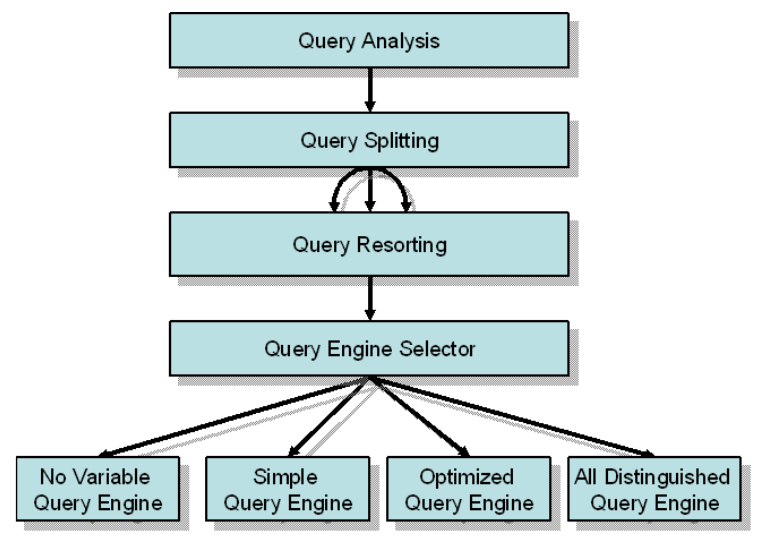
\includegraphics{bilder/infres_pellet_queryengine.png}}}
    \caption{Ablauf Beantwortung einer Anfrage in der Abox Query-Engine.\label{fig:pellet_queryengine_komponenten}\protect\footnotemark}
\end{figure}
\footnotetext{\cite[S. 11]{sirin:pellet05}}

\subsubsection{Gültigkeitsprüfung bezüglich OWL-DL}
\label{ssubsection:inferenz_pellet_owldl}
Werkzeuge zur Modellierung und Export von Ontologien im OWL-Format, bieten häufig Charakteristika von OWL-full zur Modellierung an. Bei der Gültigkeitsprüfung einer Ontologie wird diese analysiert und gegebenenfalls mittels Heuristiken von OWL-full in OWL-DL umgewandelt.

Diese Umwandlung ist jedoch nur in gewissen Fällen möglich, so z.B.\ gleiche Bezeichnung von Klassen, Eigenschaften und Individuen, andernfalls werden die OWL-full Charakteristika ignoriert oder der Prozess wird komplett abgebrochen.

\subsection{Behandlung von Regeln in Pellet}
\label{subsection:inferenz_pellet_swrl}
Pellet ermöglicht die Verwendung von in SWRL formulierten Regeln zum Ziehen von Schlüssen. Damit die in der Wissensdatenbank gespeicherten Konzepte in den Regeln verfügbar sind, wird das $\mathcal{AL}$-Log-Framework eingesetzt. Dieses verbindet Beschreibungslogik mit Regeln.~\cite[Seiten 4 und 5]{sirin:pellet07} $\mathcal{AL}$-Log ist ein integriertes System zur Repräsentation von Wissen, welches auf der Beschreibungslogik $\mathcal{AL}$ und der deduktiven Datenbanksprache Datalog basiert.~\cite{allog} Bei $\mathcal{AL}$ handelt es sich um eine minimale Sprache der Beschreibungslogik, Details siehe~\cite[Seite 51]{dl:baader2003}. Als Implementation des $\mathcal{AL}$-Log-Frameworks nutzt Pellet einen Datalog-Reasoner.~\cite[Seiten 4 und 5]{sirin:pellet07}

Bei Datalog handelt es sich um eine deklarative Logiksprache, in welcher jede Formel eine funktionsfreie Hornklausel ist. Im Unterschied zu Prolog muss jede Variable, die im Kopf einer Klausel vorkommt, auch im Körper der Klausel vorkommen. Weiter spielt die Reihenfolge, in welcher die Klauseln angegeben werden, keine Rolle. Alle Anfragen terminieren und jede mögliche Antwort wird ausgegeben.~\cite{datalog}

In der Pellet-Implementation wird das $\mathcal{AL}$-Log-Framework dahingehend erweitert, dass es die Beschreibungslogik $\mathcal{SHOIQ}(\mathcal{D})$ nutzen kann. Die Erweiterung erlaubt zudem die Verwendung von OWL-Datentypen und SWRL-Funktionen im Körper von Datalog-Regeln.~\cite[Seite 5]{sirin:pellet07}

\subsection{Optimierungen}
\label{subsection:inferenz_pellet_opti}
Dieser Abschnitt basiert, sofern nicht anders im Text vermerkt, auf~\cite[Seiten 16 bis 19]{sirin:pellet05}

Beschreibungslogiken, wie $\mathcal{SHOIQ}(\mathcal{D})$ haben im schlechtesten Fall eine sehr hohe Komplexität. Daher unterscheidet sich die effektive Implementation einer solchen sehr stark von deren Design bzw. Theorie.

Um dennoch akzeptable Leistungen beim Ziehen von Schlüssen mittels Beschreibungslogik zu erhalten, nutzen moderne Reasoner verschiedene Arten von Optimierungen, so z.B.:

\begin{itemize}
    \item \textbf{Normalisierung und Vereinfachung}\\
        Alle Konzepte der Wissensdatenbank werden in eine Form gebracht, so dass Widersprüche möglichst früh während der Tableaux-Erweiterung erkannt werden können. Sie werden also in die Normalform gebracht.\\
        Die Vereinfachung erkennt offensichtliche Fehler während der Normalisierung. Weiter werden mehrfache Vorkommen eines Konzeptes eliminiert.

    \item \textbf{Tbox-Absorption}\\
        Bei dem Prozess der Tbox-Absorption wird versucht gleiche Konzepte (GCI --- General Concept Inclusion) zu eliminieren, indem diese mit Definitionen atomarer Konzepte ersetzt werden.

    \item \textbf{Dependency-directed Backjumping}\\
        Der Prozess des dependency-directed Backjumpings eliminiert unproduktive Backtracking-Suchen, indem er herausfindet welche Verzweigungspunkte Konflikte verursachen. Er springt dann zurück und überspringt dabei diese Punkte ohne nach Alternativen zu suchen.
\end{itemize}

Weitere Verfahren zur Optimierung sowie mehr Details finden sich unter~\cite[S. 17 bis 19]{sirin:pellet05}.


\subsection{Unterschiede zu Prolog}
\label{}
Datalog: in kopf verwendete variablen müssen auch im körper vorkommen. in prolog nicht. anfragen terminieren in datalog, jede mögliche antwort wird zurückgegeben, in prolog ist dies nicht gegeben, endlosschleifen möglich, die reihenfolge von regeln spielt eine rolle.~\cite[Seite 175]{laemmel}

Ein weiterer, fundamentaler Unterschied ist die Art, wie Schlüsse gezogen werden. Prolog basiert grundsätzlich auf dem SLD-Resolutionsverfahren~\citep[Details siehe][Seite 68]{laemmel}. Im Gegensatz dazu kommt bei dem eingesetzten Reasoner der Tableau-Algorithmus zum Einsatz.

So ist es in Prolog ohne Weiteres möglich so genannte Constraint-Satisfaction-Probleme (Bedingungserfüllungsprobleme) zu lösen~\citep[Details siehe][Seite 148]{laemmel}. Mit Pellet bzw. Ontologien und Regeln ist dies nicht ohne Weiteres möglich. Versuche dazu finden sich unter~\citet{xiong2008constraint},~\citet{staab2006constraint} und~\citet{bramer2007constraint}.

\noindent\rule[1ex]{\textwidth}{1pt}
\begin{wrapfigure}[14]{l}{0.1\textwidth}
    \vspace{-12pt}
    
\includegraphics[width=0.1\textwidth]{bilder/elephant.png}
\end{wrapfigure}
Das unter~\ref{lst:reasoning_seilpark} genannte Beispiel beantwortet genau die unter~\ref{sec:wissensrepFormen_Wissensnetze} gestellte Frage, wie man zum Schluss gelangt, dass das Individuum \textit{Seilpark Balmberg} in der \textit{Region} \textit{Solothurn} ist.

Wie wendet man dies jedoch an? Wie gelangt man effektiv zu dieser Information? Kann dies effektiv durch reine Folgerung erreicht werden?

Die Antwort hierzu lautet ja und nein. Modelliert man die Situation beispielsweise in Protégé und nutzt den Pellet-Reasoner zum Ziehen von Schlüssen, so würde man annehmen, dass dies der Fall ist. Rein von den Möglichkeiten her sollte der Reasoner genau dies bieten. Dies ist jedoch nicht ganz der Fall, wie in der nachfolgenden Grafik ersichtlich ist.

\begin{figure}[H]
\centering \rotatebox{0}{\scalebox{0.5}[0.5]{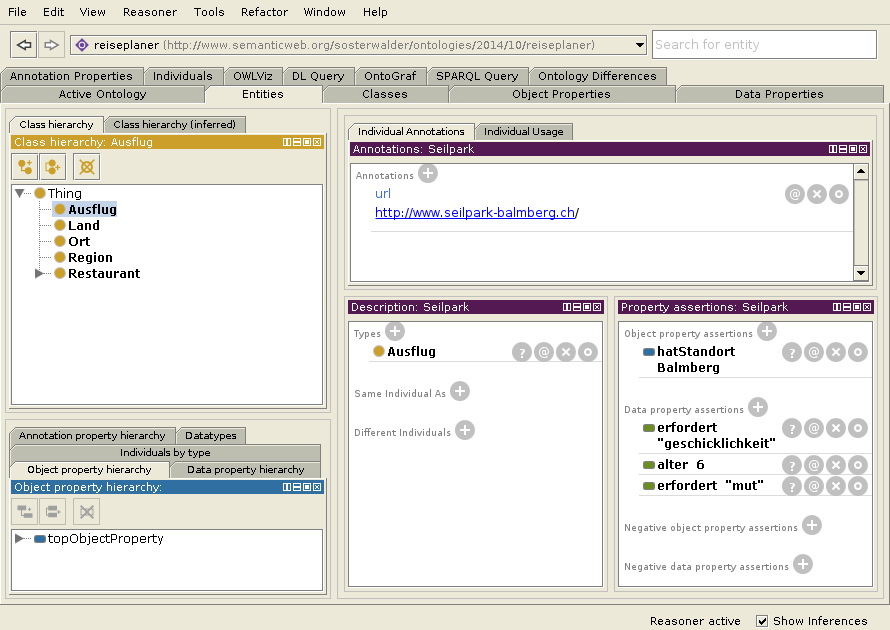
\includegraphics{bilder/inferenz_protege.png}}}
\caption{Darstellung des Individuums \textit{Seilpark Balmberg} in Protégé.\label{fig:inferenz_protege}\protect\footnotemark}
\end{figure}
\footnotetext{Eigene Darstellung mittels Stanford Protégé Version 5.0.0 beta 15}

Eine solche Folgerung ist durchaus möglich, man muss den Relationen die entsprechenden Eigenschaften, wie Symmetrie oder Transitivität, geben. Wir haben dies in unserem Fall jedoch bewusst nicht getan, da sonst Folgerungen auftreten, welche irreführend sind, so wäre dann z.B.\ ein Ort auch ein Land und umgekehrt.

Wir haben die eigentliche Folgerung mittels einer Regel in der Ontologie vorgenommen. Dies führen wir zu einem späteren Zeitpunkt noch genauer aus.

\noindent\rule[1ex]{\textwidth}{1pt}

\chapter{RDF und OWL}
\label{chap:owl_Rdf}

\section{RDF}
\label{sec:owlRdf_rdf}

Das RDF Kapitel basiert auf der Spezifikation von w3 \cite{w3rdf}.\\
Das "`Resource Description Framework"' RDF ist ein Framework um Informationen aus Ressourcen zu formulieren. Ressourcen können Dokumente, Leute, Objekte aber auch abstrakter Inhalt darstellen. Mit RDF können Informationen im Web von Anwendungen verarbeitet werden, anstatt sie nur anzuzeigen. RDF bietet ein gemeinsames Framework um die Informationen zwischen Anwendungen auszutauschen ohne Bedeutung zu verlieren. 

RDF ist die Grundlage für Sematic Web, welches seine flexibilität ausnützt. Alle Daten im Semantic Web werden in RDF abgebildet. Wichtig dabei ist, dass RDF es ermöglicht Daten zu verknüpfen. Dies führt dazu, dass zu einer Ressource mehr Informationen zusammen getragen werden.\cite{cambSemRDF}

%\subsection{Einsatzgebiete}
%\label{sec:logischeProgrammierung_herkunft_einsatz}
\subsection{RDF Data Model}
\label{subsec:owlRdf_rdf_dataModel}
Die Informationen werden in RDF als Aussagen abgebildet. Der Aufbau dieser  ist immer gleich und weist die folgende Struktur eines Tripels auf:

\noindent\hspace*{15mm}<Subjekt><Prädikat><Objekt>

Eine RDF Aussage bildet eine Beziehung zwischen zwei Ressourcen (Entitäten) ab. 
Subjekt und Objekt stellen die zwei Ressourcen dar. Das Prädikat repräsentiert die Beziehung zwischen den zwei Ressourcen Subjekt und Objekt. Die Beziehung wird in RDF als Property abgebildet. 
 
\noindent\hspace*{15mm} <Eine Programmiersprache> <hat> <ein Programmierparadigma>


Eine Entität kann in mehreren Tripeln referenziert werden. Es ist zudem möglich eine Ressource in einer Aussage als Objekt und in einer Anderen als Subjekt zu verwenden. dies ermöglicht es, Verbindungen zwischen mehreren Tripeln herzustellen. Dies ist ein wichtiger Teil von RDF.

Tripel werden in sogenannte RDF Graphen abgebildet. Diese bestehen aus Knoten und Pfeilen. die Subjekte und die Objekte werden als Knoten, die Prädikate als Pfeile dargestellt. Genaueres dazu findet sich im Kapitel \nameref{chap:graph_data}



TODO Bildli von Unserer Ontologie

Es gibt drei Typen von RDF Daten, welche in Tripeln auftreten, IRIs (oder Ressource Knoten) Literale und Blank (Leere) Knoten.

\subsubsection{IRIs (International Resource Identifier)}
\label{sec:owlRdf_rdf_dataModel_iris}
Wie der Name schon sagt, stellt ein IRI  eine Ressource dar. Dabei handelt es sich um einen globalen Identifier, IRIS können also von verschiedenen Nutzern wiederverwendet werden. Es gibt verschieden Formen von IRIs, so zum Beispiel die URLs welche als Web Adresse verwendet werden. Eine Andere Form der IRI bietet eine Kennung für eine Ressource ohne den Standort oder den Zugriff preiszugeben.% IRIs sind im RFC 3987 spezifiziert.

\noindent\hspace*{15mm}IRIs kann in allen drei Positionen eines Tripels auftreten.

\subsubsection{Literale Knoten}
\label{sec:owlRdf_rdf_dataModel_literal}
Der Begriff Literal wird als Synonym für Wert verwendet. Es handelt sich bei Literalen also um Basicwerte die nicht IRIS sind. Literale können Strings, Datumswerte oder auch Nummern sein. Um die Werte richtig zu interpretieren, haben Literale einen Datentyp zugeordnet. Ein String kann zusätzlich eine Sprache zugewiesen haben.

Literale können in einem Tripel nur als Objekt verwendet werden.

\subsubsection{Blank Nodes}
\label{sec:owlRdf_rdf_dataModel_blankNodes}
Ein leerer Knoten stellt eine Ressource ohne URI dar. Der Vorteil dieser Knoten ist, dass es keinen globalen Identifier braucht. Leere Knoten können mit einer einfachen Variable in der Algebra verglichen werden. Sie bilden ein Objekt ab, wobei der Wert zweitrangig ist. 

\noindent\hspace*{15mm} Leere Knoten können in einem Tripel in der Subjekt oder der Objekt Position stehen.


\subsubsection{Multiple Graphs}
\label{sec:owlRdf_rdf_dataModel_multipleGraphs}

TODO: brauchts das?

\subsection{RDF Vokabular}
\label{sec:owlRdf_rdf_voca}
RDF wird typischerweise in Kombination mit Vokabular und Konventionen verwendet, welche Semantische Daten zu Ressourcen zur Verfügung stellen.

Um das Vokabular von RDF zu zu definieren wird die RDF Schema Sprache unterstützt. Diese ermöglicht semantische Eigenschaften der RDF Daten zu definieren. Es kann damit festgelegt werden, welche Ressourcen an welcher Position verwendet werden.

so verwendet RDF zum Beispiel die Bezeichnung der Klasse um zu kategorisieren. Die Beziehungen zwischen Instanzen werden in Propertys abgebildet. Mit RDF können auch Hierarchien im Bereich der Klassen aber auch der Eigenschaften gebildet werden. Ausserdem können auf Objekten und Subjekten Typeinschränkungen vorgenommen werden.

\begin{center}
	\begin{table}[H]
	 \centering
		\caption{Schematische Konstrukte}	
			\begin{tabular}{|l|l|l|} \toprule
			\textbf{Konstrukt}  & \textbf{Syntaktische Form} & \textbf{Beschreibung} \\ \midrule
				Class (eine Klasse) & C rdf:type; rdfs:Class& C (eine Ressource) ist eine RDF Klasse \\  \midrule		
				Property (Eine Klasse) & P rdf:type rdf:Property & P (eine Ressource) ist eine RDF Property\\  \midrule		
				type (eine Eigenschaft) & I rdf:type C &I (eine Ressource) ist eine Istanz von C (einer Klasse)\\  \midrule
subClassOf (eine Eigenschaft) & C1 rdfs:subClassOf C2 & C1 (eine Klasse) ist Subklasse von C2 \\  \midrule
subProptertyOf (eine Eigenschaft) & P1 rdfs:subProptertyOf P2 & P1 (eine Eigenschaft) ist Sub-Property von P2 \\  \midrule
domain (eine Eigenschaft) & P rdfs:domain C & Domäne von P (einer Eigenschaft) ist C (eine Klasse) \\  \midrule			
range (eine Eigenschaft) & P rdfs:range C & Bereich von P (einer Eigenschaft) ist C (eine Klasse) \\  \bottomrule
			\end{tabular}
		\label{tab:SchematischeKonstrukte}
	\end{table}
\end{center}

TODO: Writing RDF graphs wird hier noch ausführlich beschrieben. Nach dem Kapital Graphen Modellierung entscheiden was davon noch nötig ist und einfügen.

\section{OWL}
\label{sec:owlRdf_owl}

Bei OWL (Web Ontology Language) und OWL2 handelt es sich um die Ontologie Sprache für das Semantische Web.\cite{cambSemOWL} Also um eine Sprache um Ontologien auszudrücken. Wie bei RDF wurde OWL Entwickelt um Informationen nicht nur anzuzeigen sondern auch zu verarbeiten. Durch zusätzliches Vokabular wie zum Beispiel Beziehungen zwischen Klassen und erweiterte formale Semantik hat der Benutzer mehr Möglichkeiten als bei RDF oder auch XML. \\OWL basiert aber technische gesehen auf der RDF Syntax. %Die Verknüpfung und Darstellung von Termen in Vokabularien und deren Verknüpfungen wird in OWL als Ontologie bezeichnet. Besonders an OWL ist ausserdem, dass es maschineninterpretierbare Inhalt im Web repräsentieren.  

\subsection{OWL Syntax}
\label{subsec:owlRdf_owl_syntax}
Für OWl stehen verschiedene Schreibweisen zur Verfügung, welche für verschieden Anwendungszwecke gedacht sind:
\begin{itemize}
	\item RDF/XML Syntax für OWL: entspricht RDF/XML Syntax mit einer speziellen Übersetzen für OWL Konstrukte. Dabei handelt es sich um die einzige Syntax, welche von allen OWL 2 Tools unterstützt werden soll.
	\item OWL/XML Syntax: XML Syntax für OWL
	\item Functional-Style Syntax: Zur Vereinfachung von Spezifikationszweck; Unterstützt Grundlagen zur Implementation von OWL 2 wie APIs und Reasoners
	\item Turtle Syntax: TODO 
	\item Manchester Syntax: Vereinfacht das lesen für nicht logik affine Leser.
\end{itemize}
es gibt Werkzeuge, welche die Übersetzung zwischen den verschiedenen Schreibweisen vornimmt.

Bei OWL2 handelt es sich nicht um eine Schemasprache. Im Gegensatz zu XML beschreibt OWL nicht wie ein Dokument aufgebaut sein muss. So kann auch nicht vorgeschrieben werden, das ein bestimmtes Element vorhanden sein muss.


\subsection{Wissen modellieren}
\label{subsec:owlRdf_owl_wissenModellieren}
OWL bildet Wissen einer Domaine ab. Es handelt sich also um eine Wissensbasierte Repräsentationssprache.

Um das Abbilden von Wissen zu erklähren sollen hier

Grund Notationen:
- Axion Basis Statement 
- Entitäten: Elemente für Real world Obejkte
- Expressions: Kombination aus Entitäten um komplexe Beschreibungen zu machen


Keine Möglichkeit das sämtliche Aspekte des Menschlichen Wissen abzubilden. starke modellierungssprache. -> Ergebnis Ontologie.
Basic Propositione wie "`Prolog verwendet Unifikation"' -> Stücke des Wissens -> Aussagen werden Axiome genant.

OWL Aussage je nach Sachlage wahr oder falsch. -> Unterschied zu Entitäten und Expressions.

Ein Mensch kann Schlussfolgern. Wenn eine Aussage war ist, ist die andere Auch war. A für zu B

-> OWL Tools: Reasoners: Kann Konsequenzen ermitteln. Der weg wie Axiome interagieren kann schwer zu versthen sein. so ist es eine Stärke und eine Schwäche von OWL. -> kann Infos aufdecken welche ein Mensch nicht sieht. Schwäche -> schwierig für den Mensche die unmittelbar wirkung vorherzusehen

Entitäten:
 wesentliche Bestanteile einer Aussage wie zb Prolog, die Relation verwendet werden Entitäten genannt. Konkrete objekte als Individuals; Categorien als Klassen; Beziehunge als Properties; ObjektProperties (wert zu objekt: Person zu einem Ehegatten) und Datatypproperty ( Datenwert zu Objekt: alter zu einer Person); AnnotationPropertie: Information zu konkrete Ontologie (Autor und erzeugungsdatum eines Axioms)

Expression: 
enitäten könen mithilfe eines Construktors kombiniert werden. Bsp Klasse Prolog + Klasse Unifikation.
-> kann als neue Entität angesehen werden
Expressionsprache für Klassen ist sehr mächtig; Expressionsprache für Properties ist schwächer. TODO: Wenden wir das richtig an?

ab hier weiter: 4 Classes, Properties, and Individuals – And Basic Modeling With Them



\subsection{OWL Untersprachen}
\label{subsec:owlRdf_owl_Untersprachen}
TODO: OWL ist in drei Untersprachen gegliedert. Jede dieser Sprachen wurde für Verwendung durch verschiedene Gruppen entwickelt. Dabei handelt es sich um OWL Lite, OWL DL und OWL Full. Die neue Version OWL2 unterscheidet zusätzlich in OWL2 QL, OWL2 EL und OWL2 RL. Dabei handelt es sich um weitere Unterklassen von OWL2 DL welche wiederum eine Untersprache von OWL2 Full ist.


%w3c
%http://www.w3.org/TR/2012/REC-owl2-primer-20121211/
%http://www.w3.org/2001/sw/wiki/OWL

%http://www.w3.org/TR/2014/NOTE-rdf11-primer-20140624/

% Einträge im Verzeichnis erscheinen lassen ohne hier eine Referenz einzufügen
%\nocite{kopka:band1}

\chapter{SPARQL}
\label{chap:sparql}
Im letzten Kapitel wurde aufgezeigt, wie Inferenz in einer Ontologie mittels der Regelsprache SWRL vollumfänglich genutzt werden kann.

Wie können Informationen aus der Ontologie und den darauf basierenden Inferenzen abgefragt werden?\\
Mit SPARQL --- einer Abfragesrprache --- ist es möglich.

Im folgenden Kapitel, welches, sofern nicht anders vermerkt, auf~\cite{w3sparql_querylang} basiert, stellen wir diese Abfragesprache vor.

Bei SPARQL handelt es sich sich um eine Abfragesprache für RDF.\@ Sie erlaubt es, Abfragen in mehreren Datenquellen vorzunehmen. Dabei werden Anfragen über Graphen vollzogen, auch entlang derer Konjunktionen und Disjunktionen. SPARQL unterstützt weiter Aggregation, Unterabfragen, Negation sowie die Nutzung von Ausdrücken als Werte.

Resultate sind entweder eine Menge von Ergebnissen oder RDF-Graphen.

% (vgl.~\cite[Abstract]{w3sparql_querylang})

\noindent\rule[1ex]{\textwidth}{1pt}
\begin{wrapfigure}[7]{l}{0.1\textwidth}
    \vspace{-12pt}
    
\includegraphics[width=0.1\textwidth]{bilder/owl.png}
\end{wrapfigure}
Kennt man die Abfragesprache SQL, so erscheint SPARQL auf den ersten Blick recht ähnlich --- der Name lässt dies bereits vermuten. Dies ist nur teilweise der Fall. Klauseln wie \textit{SELECT} und \textit{WHERE} sind ähnlich. In SPARQL gibt es jedoch keine \textit{FROM}-Klausel.\\
Der Hauptunterschied zwischen SPARQL und SQL ist jedoch die Verwendung von Variablen.  Diese werden in SPARQL in der Regel  bei jeder Abfrage verwendet. Abfragen ohne Variablen kommen in der Praxis (gemäss unserer Erfahrung) eher selten vor.\\
SQL enthält in der Regel sehr wenig Variablen.

\noindent\rule[1ex]{\textwidth}{1pt}

Eine SPARQL-Abfrage besteht aus folgenden Komponenten:
\begin{itemize}
    \item Einem oder mehreren Namespaces
    \item Variablen
    \item Einem (Teil-) Graphen
    \item Einer Menge von Gruppierungen und Aggregationen
    \item Einer Menge von Modifikatoren
    \item Abfragearten
    \item Ausdrücken und Wertevergleichen
\end{itemize}
% (vgl.~\cite[18.1.10 SPARQL Query]{w3sparql_querylang})

\noindent\rule[1ex]{\textwidth}{1pt}
\begin{wrapfigure}[2]{l}{0.1\textwidth}
    \vspace{-19pt}
    
\includegraphics[width=0.1\textwidth]{bilder/owl.png}
\end{wrapfigure}
Für die Praxis besteht eine SPARQL-Abfrage in der Regel aus \textit{Namespaces}, einer \textit{SELECT}-Klausel, einer \textit{WHERE}-Klausel sowie \textit{Modifikatoren}.\\

\noindent\rule[1ex]{\textwidth}{1pt}

\section{Beispiel einer SPARQL Abfrage}
\label{sec:sparql_beispiel}

Gegeben sei die folgende Datenbasis:
\lstset{caption={Einfache Datenbasis direkt in SPARQL\protect\footnotemark},captionpos=b}
\begin{lstlisting}
   <http://example.org/book/book1> <http://purl.org/dc/elements/1.1/title> "SPARQL Tutorial".
\end{lstlisting}
\footnotetext{\cite[2.1 Writing a Simple Query]{w3sparql_querylang}}

Die Datenbasis beinhaltet das Objekt \textit{book1} mit dem Attribut \textit{title}, welches den Wert \textit{``SPARQL Tutorial''} enthält.

Möchte ich nun den Titel des Buches abfragen, so kann ich folgende Abfrage verwenden:
\lstset{caption={Beispiel einer einfachen SPARQL-Abfrage\protect\footnotemark},captionpos=b}
\begin{lstlisting}
    SELECT
        ?title
    WHERE {
        <http://example.org/book/book1> <http://purl.org/dc/elements/1.1/title> ?title .
    }
\end{lstlisting}
\footnotetext{\cite[2.1 Writing a Simple Query]{w3sparql_querylang}}

Sie ergibt folgendes Resultat:
\noindent\hspace*{15mm}
\begin{table}[h]
    \centering
    \begin{tabular}{|l|}
        \hline
        \multicolumn{1}{|c|}{\textbf{title}} \\ \hline
        ``SPARQL Tutorial''                    \\ \hline
    \end{tabular}
    \caption{Resultat einer einfachen SPARQL-Abfrage\protect\footnotemark}
\end{table}
\footnotetext{\cite[2.1 Writing a Simple Query]{w3sparql_querylang}}

\section{Namespaces}
\label{sec:sparql_namespaces}

SPARQL ist eine Abfragesprach für RDF, das seinerseits auf XML basiert. Dadurch sind XML-Namespaces auch in SPARQL verfügbar. Bei Namespaces handelt es sich um Referenzen auf andere XML-basierte Dokumente, welche modular genutzt werden können.\\
Ein Namespace besteht aus einem Kürzel (welches auch leer sein kann), sowie aus der kompletten Adresse der Ressource (vgl.~\cite[2.1 Introduction]{w3rdf_syntax}).

\lstset{language=XML,
  caption={Beispiel von Namespaces in RDF\protect\footnotemark},
  frame=L,
  basicstyle=\small\normalfont\sffamily,  % the size of the fonts that are used for the code
  stepnumber=1,                           % the step between two line-numbers.
                                          % If it is 1 each line will be numbered
  numbersep=10pt,                         % how far the line-numbers are from the code
  tabsize=2,                              % tab size in blank spaces
  extendedchars=true,                     %
  breaklines=true,                        % sets automatic line breaking
  captionpos=b,                           % sets the caption-position to bottom
  mathescape=true,
  showspaces=false,                       % Leerzeichen anzeigen ?
  showtabs=false,                         % Tabs anzeigen ?
  xleftmargin=17pt,
  framexleftmargin=17pt,
  framexrightmargin=17pt,
  framexbottommargin=5pt,
  framextopmargin=5pt,
  showstringspaces=false                  % Leerzeichen in Strings anzeigen ?
  belowcaptionskip=5em,
  belowskip=3em,
  aboveskip=3em
 }
\begin{lstlisting}
$\textless$rdf:RDF xmlns:rdf="http://www.w3.org/1999/02/22-rdf-syntax-ns#"
         xmlns:dc="http://purl.org/dc/elements/1.1/"
         xmlns:ex="http://example.org/stuff/1.0/"$\textgreater$
\end{lstlisting}
\footnotetext{\cite[2.6 Completing the Document: Document Element and XML Declaration]{w3rdf_syntax}}

\section{Variablen}
\label{sec:sparql_variablen}
Bei Abfragen unterstützt SPARQL die Verwendung von Variablen. Diese können dabei an einer beliebigen Stelle, wie bei (Teil-) Graphen, Gruppierungen, Aggregationen und Modifikatoren eingesetzt werden.\\
Die Variablen dienen als Platzhalter für abzufragende Objekte, Subjekte und Prädikate. Variablen beginnen entweder mit einem Dollarzeichen \textit{\$} oder einem Fragezeichen \textit{?}, welche selbst nicht Teil der Variable sind.

\lstset{caption={Beispiel einer SPARQL Abfrage mit den Variablen \textit{?object}, \textit{?predicate} und \textit{?subject}.},captionpos=b}
\begin{lstlisting}
    SELECT DISTINCT
        *
    WHERE {
      ?object ?predicate ?subject
    }
    LIMIT
        10
\end{lstlisting}

Wird obige Anfrage auf einen SPARQL-Endpunkt, wie z.B. \textit{http://dbpedia.org/}, angewendet, so ergibt dies folgendes Resultat:
\noindent\hspace*{15mm}
\begin{table}[h]
    \centering
    \begin{tabular}{l|l|l|}
        \hline
        \multicolumn{1}{|l|}{\textbf{object}}                                & \textbf{predicate}                               & \textbf{subject}                                  \\ \hline
        \multicolumn{1}{|l|}{http://dbpedia.org/ontology/acceleration}      & ... rdf-syntax-ns\#type & ... owl\#FunctionalProperty \\ \hline
        \multicolumn{1}{|l|}{http://dbpedia.org/ontology/torqueOutput}      & ... rdf-syntax-ns\#type & ... owl\#FunctionalProperty \\ \hline
        \multicolumn{1}{|l|}{http://dbpedia.org/ontology/birthDate}         & ... rdf-syntax-ns\#type & ... owl\#FunctionalProperty \\ \hline
        \multicolumn{1}{|l|}{http://dbpedia.org/ontology/birthYear}         & ... rdf-syntax-ns\#type & ... owl\#FunctionalProperty \\ \hline
        \multicolumn{1}{|l|}{http://dbpedia.org/ontology/deathDate}         & ... rdf-syntax-ns\#type & ... owl\#FunctionalProperty \\ \hline
        \multicolumn{1}{|l|}{http://dbpedia.org/ontology/deathYear}         & ... rdf-syntax-ns\#type & ... owl\#FunctionalProperty \\ \hline
        \multicolumn{1}{|l|}{http://dbpedia.org/ontology/diameter}          & ... rdf-syntax-ns\#type & ... owl\#FunctionalProperty \\ \hline
        \multicolumn{1}{|l|}{http://dbpedia.org/ontology/displacement}      & ... rdf-syntax-ns\#type & ... owl\#FunctionalProperty \\ \hline
        \multicolumn{1}{|l|}{http://dbpedia.org/ontology/height}            & ... rdf-syntax-ns\#type & ... owl\#FunctionalProperty \\ \hline
        \multicolumn{1}{|l|}{http://dbpedia.org/ontology/latestReleaseDate} & ... rdf-syntax-ns\#type & ... owl\#FunctionalProperty \\ \hline
    \end{tabular}
    \caption{Resultat einer Abfrage des DBPedia-Endpunktes limitiert auf 10 Ergebnisse.}
\end{table}

\section{(Teil-) Graphen}
\label{sec:sparql_graph}

SPARQL basiert auf dem Matching eines (Teil-) Graphen in einem gegebenen Graphen. Dabei ist ein (Teil-) Graph eine Menge von Tripeln.

Man unterscheidet zwischen den folgenden Arten von Teilgraphen:
\begin{itemize}
\item \textit{Grundlegende Teilgraphen}

Hierbei muss eine Menge von Tripeln derjenigen im gegebenen Graphen entsprechen

\item \textit{Gruppierende Teilgraphen}

Hierbei müssen \textit{alle} Elemente einer Menge von Tripeln von grundlegenden Teilgraphen wiederum derjenigen im gegebenen Graphen entsprechen

\item \textit{Optionale Teilgraphen}

Zusätzliche Teilgraphen können die Lösungsmenge erweitern

\item \textit{Alternative Teilgraphen}

Versuch, ob zwei oder mehrere mögliche Teilgraphen denjenigen im gegebenen Graphen entsprechen

\item \textit{Teilgraphen in namensbasierten Graphen}

Versuch, ob Teilgraphen denjenigen im gegebenen, namensbasierten Graphen entsprechen
\end{itemize}

Ein grundlegender Teilgraph ist somit eine Menge von Tripeln, wobei jeder Tripel gemäss RDF-Spezifikation immer aus Subjekt, Prädikat und Objekt bestehen muss (vgl.~\cite[3.1 Triples]{w3rdf}).

\lstset{caption={Beispiel eines grundlegenden Teilgraphen in SPARQL}}
\begin{lstlisting}
    ?subject ?predicate ?object.
\end{lstlisting}

\noindent\rule[1ex]{\textwidth}{1pt}
\begin{wrapfigure}[3]{l}{0.1\textwidth}
    \vspace{-16pt}
    
\includegraphics[width=0.1\textwidth]{bilder/owl.png}
\end{wrapfigure}
Ein Teilgraph wird in SPARQL immer zur Gruppierung einer Abfrage verwendet. Dies entspricht in der SQL-Sprache der \textit{WHERE}-Klausel.\\
Ein Teilgraph wird immer mit dem Punkt-Operator beendet.

\noindent\rule[1ex]{\textwidth}{1pt}

Ein gruppierender Teilgraph wird in der SPARQL-Abfrage immer mit geschweiften Klammern \textit{\{\}} umschlossen. Es ist möglich die Resultate einer Gruppierung zu filtern. Dazu wird \textit{FILTER} als Schlüsselwort verwendet. Dieses bezieht sich immer auf die Gruppierung, in welcher es steht.

\lstset{caption={Beispiel eines gruppierenden Teilgraphen mit dem \textit{FILTER}-Schlüsselwort\protect\footnotemark}}
\begin{lstlisting}
    {
        ?x foaf:name ?name.
        ?x foaf:mbox ?mbox.
        FILTER regex(?name, "Smith")
    }
\end{lstlisting}
\footnotetext{\cite[5.2.2 Scope of Filters]{w3sparql_querylang}}

Im obigem Beispiel werden alle Objekte und die Werte ihrer Attribute (\textit{name} und \textit{mbox}, welche im Namespace \textit{foaf} bezeichnet werden) abgefragt.

Dabei kann eine komplette leere Menge --- wenn keine Objekte vorhanden sind --- oder aber eine leere Teilmenge --- wenn ein Objekt z.B. nicht über die beiden Attribute \textit{name} und \textit{mbox} verfügt --- zurückgegeben werden.

Es bleiben nur Objekte zurück, welche über das Attribut \textit{foaf:name} verfügen und dessen Inhalt \textit{``Smith''} ist.

\section{Gruppierungen und Aggregationen}
\label{sec:sparql_gruppierungenaggregationen}
Aggregationen bezeichnen eine bestimmte Art der Verbindung zwischen Objekten.~\cite{wiki:aggregation} Aggregationen wenden Ausdrücke bzw. Funktionen auf eine Lösungsmenge an. Dabei enthält eine Lösung normalerweise eine einzelne Gruppe mit allen Lösungen.

Gruppierungen werden mittels \textit{GROUP BY} angegeben.

SPARQL unterstützt aktuell die Aggregationen \textit{COUNT}, \textit{SUM}, \textit{MIN}, \textit{MAX}, \textit{AVG}, \textit{GROUP\_CONCAT} und \textit{SAMPLE}.

Die Aggregation wird dann verwendet, wenn ein Resultat über eine Gruppe von Lösungen berechnet werden soll (Beispiel: Maximaler Wert einer bestimmten Variablen).

\lstset{caption={Beispiel einer Abfrage mit Gruppierung und Aggregation\protect\footnotemark}}
\lstset{language=SQL}
\begin{lstlisting}
    PREFIX books: $\textless$http://books.example/$\textgreater$
    SELECT (
        SUM(?lprice) AS ?totalPrice
    )
    WHERE {
      ?org books:affiliates ?auth .
      ?auth books:writesBook ?book .
      ?book books:price ?lprice .
    }
    GROUP BY ?org
    HAVING (SUM(?lprice) $\textgreater$ 10)
\end{lstlisting}
\footnotetext{\cite[11.1 Aggregate Example]{w3sparql_querylang}}
    
\section{Modifikatoren}
\label{sec:sparql_modifikatoren}
Abfragen mittels SPARQL generieren eine ungeordnete Menge von Lösungen. Jede dieser Lösungen stellt eine Funktion von Variablen zu RDF-Termen dar. So gewonnene Lösungen werden als Sequenz von Lösungen behandelt, zunächst ohne spezifische Ordnung.

Um eine Sequenz von Lösungen zu ordnen, werden Modifikatoren verwendet.\\
Dabei unterscheidet man zwischen folgenden Modifikatoren:

\begin{itemize}
    \item \textit{Order}

        Sortiert die Lösungen auf- oder absteigend nach einer bestimmten Variablen

    \item \textit{Projection}

        Erlaubt die Auswahl von spezifischen Variablen mittels der \textit{Select}-Klausel

    \item \textit{Distinct}

        Stellt sicher, dass die Lösungen in der Lösungsmenge einmalig sind

    \item \textit{Reduced}

        Verhindert die Elimination von Duplikaten in der Lösungsmenge

    \item \textit{Offset}

        Definiert, ab welchem Element der Lösungsmenge die gefundenen Lösungen ausgegeben werden

    \item \textit{Limit}

        Definiert die maximale Anzahl an gefundenen Lösungen, die ausgegeben werden soll

\end{itemize}

Die \textit{Modifikatoren} werden in der Reihenfolge der obigen Liste angewendet.


\section{Abfragearten}
\label{sec:sparql_abfragearten}

SPARQL unterscheidet zwischen vier Abfragearten:
\begin{itemize}
    \item \textit{SELECT}

        Liefert alle Variablen oder eine Teilmenge derselben eines Graphen

    \item \textit{CONSTRUCT}

        Liefert einen RDF-Graphen durch Substitution der Variablen in einer Menge von gegebenen Tripeln

    \item \textit{ASK}

        Liefert einen Wahrheitswert (Boolean), welcher angibt, ob die Menge von angefragten Tripeln derjenigen in dem gegebenen Graphen entspricht

    \item \textit{DESCRIBE}

        Liefert einen RDF-Graphen, welcher die gefundenen Ressourcen beschreibt
\end{itemize}

\subsection{SELECT}
\label{subsec:sparql_abfragearten_select}
Die \textit{SELECT}-Abfrageart liefert direkt Variablen und deren Belegung, in Form von Projektionen. Dabei entstehen neue Variablen-Belegungen. Die spezifischen, gewünschten Variablen werden in Form einer Liste, durch Leerzeichen getrennt, angegeben.

\lstset{caption={Beispiel der \textit{SELECT}-Abfrageart in SPARQL},captionpos=b,language=SQL}
\begin{lstlisting}
    SELECT ?a ?b ?c
    WHERE {
        ...
\end{lstlisting}

Die $ SELECT * $-Syntax ist eine Kurzschreibweise und bedeutet die Verwendung bzw.\ die Auflistung aller in der Abfrage verwendeten Variablen. Davon ausgenommen sind Variablen innerhalb von \textit{FILTER}-Anweisungen sowie Variablen, welche rechts des Minus-Operators stehen. Die Syntax darf nur verwendet werden, wenn die Abfrage keine \textit{GROUP BY}-Aggregation verwendet.
\lstset{caption={Beispiel der \textit{SELECT *} Kurzschreibweise in SPARQL},captionpos=b,language=SQL}
\begin{lstlisting}
    SELECT *
    WHERE {
    ...
\end{lstlisting}

Durch die \textit{SELECT}-Abfrageart lassen sich neuen Variablen durch Ausdrücke einführen. Diese werden mittels $(SELECT \; expr \; AS \; var)$ eingeführt.

\lstset{caption={Beispiel eines Ausdrucks der \textit{SELECT}-Abfrageart},captionpos=b,language=SQL}
\begin{lstlisting}
SELECT ?title (?p * (1 - ?discount) AS ?price)
WHERE {
...
\end{lstlisting}


\subsection{CONSTRUCT}
\label{subsec:sparql_abfragearten_construct}
Die \textit{CONSTRUCT}-Abfrageart gibt als Antwort einen einzigen, durch eine Vorlage definierten RDF-Graphen zurück: Jede Variable der Abfrage wird durch die passende Lösung aus der Lösungssequenz ersetzt. Die Lösungsmenge wird schliesslich durch Vereinigung der Tripel auf einen einzigen RDF-Graphen reduziert.

\lstset{caption={Beispiel einer SPARQL-Abfrage unter Nutzung der \textit{CONSTRUCT}-Abfrageart\protect\footnotemark},captionpos=b}
\begin{lstlisting}
PREFIX foaf:    $\textless$http://xmlns.com/foaf/0.1/$\textgreater$
PREFIX vcard:   $\textless$http://www.w3.org/2001/vcard-rdf/3.0#$\textgreater$
CONSTRUCT   { $\textless$http://example.org/person#Alice$\textgreater$ vcard:FN ?name }
WHERE       { ?x foaf:name ?name }
\end{lstlisting}
\footnotetext{\cite[16.2 CONSTRUCT]{w3sparql_querylang}}

Die obige Abfrage erzeugt folgende Ausgabe:
\lstset{caption={Beispiel der Ausgabe einer SPARQL-Abfrage unter Nutzung der \textit{CONSTRUCT}-Abfrageart\protect\footnotemark},captionpos=b}
\begin{lstlisting}
@prefix vcard: $\textless$http://www.w3.org/2001/vcard-rdf/3.0#$\textgreater$ .

$\textless$http://example.org/person#Alice$\textgreater$ vcard:FN "Alice" .
\end{lstlisting}
\footnotetext{\cite[16.2 CONSTRUCT]{w3sparql_querylang}}

Entsteht bei diesem Vorgang ein ungültiges Tripel, wird dieses nicht im Ausgabegraphen angezeigt.\\
Enthält die Vorlage eines Graphen Tripel ohne Variablen, erscheinen diese dennoch im Ausgabegraphen.

\lstset{caption={Beispiel einer SPARQL Abfrage mit Nutzung der \textit{CONSTRUCT}-Abfrageart unter Verwendung leerer Knoten\protect\footnotemark},captionpos=b}
\begin{lstlisting}
PREFIX foaf:    $\textless$http://xmlns.com/foaf/0.1/$\textgreater$
PREFIX vcard:   $\textless$http://www.w3.org/2001/vcard-rdf/3.0#$\textgreater$

CONSTRUCT { ?x  vcard:N _:v .
            _:v vcard:givenName ?gname .
            _:v vcard:familyName ?fname }
WHERE
 {
    { ?x foaf:firstname ?gname } UNION  { ?x foaf:givenname   ?gname } .
    { ?x foaf:surname   ?fname } UNION  { ?x foaf:family_name ?fname } .
 }
\end{lstlisting}
\footnotetext{\cite[16.2.1 Templates with Blank Nodes]{w3sparql_querylang}}

Die obige Abfrage erzeugt folgende Ausgabe:
\lstset{caption={Beispiel der Ausgabe einer SPARQL Abfrage mit Nutzung der \textit{CONSTRUCT}-Abfrageart unter Verwendung leerer Knoten\protect\footnotemark},captionpos=b}
\begin{lstlisting}
@prefix vcard: $\textless$http://www.w3.org/2001/vcard-rdf/3.0#$\textgreater$ .

_:v1 vcard:N         _:x .
_:x vcard:givenName  "Alice" .
_:x vcard:familyName "Hacker" .

_:v2 vcard:N         _:z .
_:z vcard:givenName  "Bob" .
_:z vcard:familyName "Hacker" .
\end{lstlisting}
\footnotetext{\cite[16.2.1 Templates with Blank Nodes]{w3sparql_querylang}}

\subsection{ASK}
\label{subsec:sparql_abfragearten_ask}
Die \textit{ASK}-Abfrageart beantwortet in der Ausgabe, ob eine Lösung für die gegebene Abfrage existiert.

Gegeben sei die folgende Datenbasis:
\lstset{caption={Einfache Datenbasis direkt in SPARQL\protect\footnotemark},captionpos=b}
\lstset{language=XML}
\begin{lstlisting}
@prefix foaf:       $\textless$http://xmlns.com/foaf/0.1/$\textgreater$ .

_:a  foaf:name       "Alice" .
_:a  foaf:homepage   $\textless$http://work.example.org/alice/$\textgreater$ .

_:b  foaf:name       "Bob" .
_:b  foaf:mbox       $\textless$mailto:bob@work.example$\textgreater$ .
\end{lstlisting}
\footnotetext{\cite[16.3 ASK]{w3sparql_querylang}}

Wird nun folgende Abfrage getätigt:
\lstset{caption={Beispiel einer SPARQL-Abfrage mit Nutzung der \textit{ASK}-Abfrageart\protect\footnotemark},captionpos=b}
\lstset{language=XML}
\begin{lstlisting}
    PREFIX foaf:    $\textless$http://xmlns.com/foaf/0.1/$\textgreater$
    ASK  { 
        ?x foaf:name  "Alice"
    }
\end{lstlisting}
\footnotetext{\cite[16.3 ASK]{w3sparql_querylang}}
So antwort das System: $true$, da die Datenbasis ein Individuum mit dem Attribut $foaf:name$ enthält, dessen Wert $``Alice''$ ist.

\subsection{DESCRIBE}
\label{subsec:sparql_abfragearten_describe}
Bei der \textit{DESCRIBE}-Abfrageart antwortet das System mit einem RDF-Graphen, der Informationen in Form von RDF-Daten über Ressourcen enthält. Als Ressourcen kommen entweder \textit{IRI}s oder Variablen in Betracht.

\lstset{caption={Beispiel der \textit{DESCRIBE}-Abfrageart in SPARQL},captionpos=b,language=SQL}
\begin{lstlisting}
    DESCRIBE
        ?a ?b ?c
    WHERE {
    ...
\end{lstlisting}

Die $ DESCRIBE * $-Syntax ist die Kurzschreibweise und bedeutet die Verwendung bzw.\ die Auflistung aller in der Abfrage verwendeten Variablen.
\lstset{caption={Beispiel der \textit{DESCRIBE *} Kurzschreibweise in SPARQL},captionpos=b,language=SQL}
\begin{lstlisting}
DESCRIBE *
WHERE {
...
\end{lstlisting}

\section{Ausdrücke und Wertevergleiche}
\label{sec:sparql_ausdruecke}
In SPARQL kann jede Abfrage in SPARQL mit einem Filter versehen werden. Dabei wird versucht ein bestimmtes Muster (durch Beschränkungen) auf Graphen anzuwenden um so die Graphen einzuschränken (filtern).

Jedes RDF-Literal kann durch einen bestimmten Datentyp definiert sein, wie zum Beispiel Wahrheitswerte (Boolean) oder Datum und Uhrzeit (DateTime). Der Filter in SPARQL erlaubt dabei den Wertevergleich auf typisierte RDF-Literale. Die dabei verwendeten Operanden und Datentypen finden sich unter den Webseiten~\href{http://www.w3.org/TR/xpath-functions/}{w3.org}\footnote{\url{http://www.w3.org/TR/xpath-functions/}} und~\href{http://www.w3.org/TR/sparql11-query/\#operandDataTypes}{w3.org}\footnote{\url{http://www.w3.org/TR/sparql11-query/\#operandDataTypes}}.

Eine SPARQL-Abfrage unter Verwendung eines Filters kann wie folgt aussehen:
\lstset{caption={Beispiel einer einfachen SPARQL-Abfrage unter Verwendung eines Filters},captionpos=b}
\begin{lstlisting}
    ...
    SELECT
        ?book, ?amount
    WHERE {
      ?book :isInLibrary :BerneUniversityLibrary
      ?book :hasAmount ?amount
      FILTER (?amount $\textgreater$ xsd:integer(10))
    }
\end{lstlisting}
In diesem Beispiel wird eine Datenbank nach mehrfachen Vorkommen (mindestens 10 Mal) eines Buchexemplares in der Bibliothek der Universität Bern abgefragt. Die Anzahl der Exemplare eines Buches wird durch die Variable $?amount$ zurückgegeben.

Ist man in obigem Beispiel nicht sicher, welchem Datentyp die Variable $?amount$ entspricht, kann man die Funktionalität zur Umwandlung (Casting, Typenumwandlung) von Variablen nützen:
\lstset{caption={Beispiel einer einfachen SPARQL-Abfrage unter Verwendung eines Filters mit Typenumwandlung},captionpos=b}
\begin{lstlisting}
    ...
    SELECT
        ?book, ?amount
    WHERE {
      ?book :isInLibrary :BerneUniversityLibrary
      ?book :hasAmount ?amount
      FILTER (xsd:integer(?amount) $\textgreater$ xsd:integer(10))
    }
\end{lstlisting}

Die genaue Auswertung eines Filters lassen sich unter der Webseite~\href{http://www.w3.org/TR/sparql11-query/\#evaluation}{w3.org}\footnote{\url{http://www.w3.org/TR/sparql11-query/\#evaluation}}, die interne Verwendung und Auswertung von Operatoren unter der Webseite~\href{http://www.w3.org/TR/sparql11-query/\#OperatorMapping}{w3.org}\footnote{\url{http://www.w3.org/TR/sparql11-query/\#OperatorMapping}} nachlesen.

\subsection{Funktionen}
\label{subsec:sparql_ausdruecke_funktionen}

SPARQL bietet eine Vielzahl an Operatoren und Funktionen. Diese einzeln aufführen und beschreiben zu wollen, würde den Rahmen dieser Arbeit sprengen. Daher werden nur die Operatoren und Funktionen aufgeführt, welche in der vorliegenden Arbeit hauptsächlich angewendet wurden. Eine genauere Beschreibung findet sich unter der Webseite~\href{http://www.w3.org/TR/sparql11-query/\#SparqlOps}{w3.org}\footnote{\url{http://www.w3.org/TR/sparql11-query/\#SparqlOps}}.

\subsubsection{BOUND}
\label{subsec:sparql_ausdruecke_funktionen_bound}
Mittels \textit{BOUND} lässt sich prüfen, ob ein Objekt eine Wert-Bindung hat. Man kann es als eine Art der Überprüfung auf gewisse Eigenschaften bezeichnen.

Möchte man zum Beispiel wissen, welche Personen über eine Relation zu einem Datum (z.B. ihr Erfassungsdatum) haben, so bestimmt man dies mittels:
\lstset{caption={Beispiel einer simplen Ontologie zur Nutzung der \textit{BOUND}-Funktion in einer Abfrage\protect\footnotemark},captionpos=b}
\begin{lstlisting}
@prefix foaf:        $\textless$http://xmlns.com/foaf/0.1/$\textgreater$ .
@prefix dc:          $\textless$http://purl.org/dc/elements/1.1/$\textgreater$ .
@prefix xsd:          $\textless$http://www.w3.org/2001/XMLSchema#$\textgreater$ .

_:a  foaf:givenName  "Alice".

_:b  foaf:givenName  "Bob" .
_:b  dc:date         "2005-04-04T04:04:04Z"^^xsd:dateTime .
\end{lstlisting}
\footnotetext{\cite[17.4.1.1 BOUND]{w3sparql_querylang}}

\lstset{caption={Beispiel einer SPARQL-Abfrage zur Nutzung der \textit{BOUND}-Funktion\protect\footnotemark},captionpos=b}
\begin{lstlisting}
    PREFIX foaf: $\textless$http://xmlns.com/foaf/0.1/$\textgreater$
    PREFIX dc:   $\textless$http://purl.org/dc/elements/1.1/$\textgreater$
    PREFIX xsd:   $\textless$http://www.w3.org/2001/XMLSchema#$\textgreater$
    SELECT
        ?givenName
    WHERE {
        ?x foaf:givenName  ?givenName .
        OPTIONAL { ?x dc:date ?date } .
        FILTER ( bound(?date) )
    }
\end{lstlisting}
\footnotetext{\cite[17.4.1.1 BOUND]{w3sparql_querylang}}

Die obige Abfrage ergibt folgendes Resultat:
\noindent\hspace*{15mm}
\begin{table}[h]
    \centering
    \begin{tabular}{|l|}
        \hline
        \multicolumn{1}{|c|}{\textbf{givenName}} \\ \hline
        ``Bob''                    \\ \hline
    \end{tabular}
    \caption{Resultat einer SPARQL-Abfrage mittels \textit{BOUND}-Filter\protect\footnotemark}
\end{table}
\footnotetext{\cite[17.4.1.1 BOUND]{w3sparql_querylang}}

Es wird nur die Person \textit{``Bob''} gefunden, da nur bei dieser Person eine Datum-Relation definiert ist.

\subsubsection{IF}
\label{ssubsec:sparql_ausdruecke_funktionen_if}
Die \textit{IF}-Funktion gibt Argumente aufgrund einer Bedingung, welche selbst auch ein Argument ist, zurück. Die Funktion verwendet drei Argumente als Parameter. Die Argumente sind:
\begin{itemize}
    \item Argument 1: Bedingung
    \item Argument 2: Rückgabewert wenn die Bedingung (Argument 1) zutrifft
    \item Argument 3: Rückgabewert wenn die Bedingung (Argument 1) nicht zutrifft
\end{itemize}

\lstset{caption={Beispiel der \textit{IF}-Funktion in SPARQL},captionpos=b,language=XML}
\begin{lstlisting}
IF(?a = 2,?b,?c)
\end{lstlisting}

In prozeduraler Programmierung ausgedrückt:
\lstset{caption={Beispiel der \textit{IF}-Funktion in SPARQL anhand prozeduraler Programmierung ausgedrückt},
    captionpos=b,
    language=Java
}
\begin{lstlisting}
if (a == 2) {
    return b;
} else {
    return c;
}
\end{lstlisting}

\subsubsection{IN}
\label{subsec:sparql_ausdruecke_funktionen_in}
Die \textit{IN}-Funktion prüft, ob ein Element in einer Liste vorkommt. Das zu prüfende Element wird der \textit{IN}-Funktion vorangestellt, danach folgt die zu prüfende Liste. Kommt das Element in der Liste vor, gibt die Funktion den Wahrheitswert $wahr$ bzw. $true$ zurück, andernfalls $falsch$ bzw. $false$.

\lstset{caption={Beispiel der \textit{IN}-Funktion in SPARQL},captionpos=b,language=SQL}
\begin{lstlisting}
2 IN (1, 2, 3) % Wahr
2 IN ()        % Falsch
\end{lstlisting}
\footnotetext{\cite[17.4.1.9 IN]{w3sparql_querylang}}
In den obigen Beispielen ist der erste Ausdruck wahr, da 2 in der gegebenen Liste von (1, 2, 3) vorkommt. Der zweite Ausdruck ist falsch, da 2 nicht in der leeren Liste () vorkommt.

Analog zur \textit{IN}-Funktion existiert die \textit{NOT IN}-Funktion. Dabei handelt es sich um die Negation der \textit{IN}-Funktion.


\noindent\rule[1ex]{\textwidth}{1pt}
\begin{wrapfigure}[7]{l}{0.1\textwidth}
    \vspace{-12pt}
    
\includegraphics[width=0.1\textwidth]{bilder/elephant.png}
\end{wrapfigure}
Wie beschrieben sind jetzt alle Komponenten vorhanden, um Ausflüge abbilden zu können, die den in~\autoref{chap:graph_data} (\nameref{chap:graph_data}) genannten Kriterien entsprechen.

In diesem Kapitel haben wir die bisher fehlende Abfragesprache abgehandelt.

Um auf das beschriebene Beispiel der Familie, welche einen Ausflug plant, zurückzukommen: Mit der nachfolgenden Abfrage gelingt es, alle Ausflüge mit den Kriterien  \textit{familienfreundlich}, \textit{regional} und \textit{actionreich} zu finden.

\begin{lstlisting}[caption={Beispiel einer Abfrage um alle familiengerechten, actionreichen und regionalen Ausflüge der Ontologie auszugeben},captionpos=b,language=SQL]
    SELECT
        *
    WHERE {
        ?object :familiengerecht true;
            :regional true;
            :action true.
    }
\end{lstlisting}

\noindent\rule[1ex]{\textwidth}{1pt}

\chapter{Schlusswort}
\label{chap:schlusswort}

In der vorliegenden Arbeit haben wir gezeigt, wie ein Knowledge-Engineer bei der Modellierung und Formalisierung einer Problemdomäne vorgehen kann. Am Beispiel Reiseplanung haben wir schrittweise ein Expertensystem aufgebaut.
% Das nachfolgenden Dokument zeigt, wie Wissen in einem wissensbasierten System abgebildet und genutzt werden
% kann. Anhand unseres Beispieles eines Reiseplaners wollen wir zeigen, welche Schritte eine Wissensmodellierung
% beinhaltet. Weiter zeigen wir formale Aspekte für die Wissensmodellierung auf, wie zum Beispiel verschiedene
% Sprachen. Aufgrund unserer Erfahrung geben wir praktische Tipps für die direkte Umsetzung.


Dieses Expertensystem beinhaltet eine semantische Datenbank, die ihrerseits auf der Basis einer Ontologie beruht.

Wichtige Erkenntniss: Es eignen sich nur Themengebiete, die aufgrund der Ontologie Inferenz und damit Schlussfolgerungen zulassen.

Andernfalls ist der Mehrwert der Ontolgie gegenüber der herkömmlichen Wissensabbildung nicht gegeben.

Während herkömmliche (relationale) Datenbaken nur Beziehungen aufzeigen, liegt der Vorteil der semantischen Datenbank in ihrer Flexibilität und Semantik (Möglichkeit den Relationen eine Bedeutung zu geben).

Nutzt eine Applikation eine semantische Datenbank als Datenmodell, erfordern Anpassungen (Modellierungen) des Datenmodelles keine Programmänderungen --- bei geschickter Programmierung.\\
Modellierungen sind z.B. das Hinzufügen, Bearbeiten oder Löschen von Entitäten (Klassen, Individuen, Relationen oder Eigenschaften).

Im Gegensatz hierzu benötigen Änderungen in relationalen Datenbanken meistens sehr aufwändige Programmänderungen.

%---------------------------------------------------------------------------

% Glossary
%---------------------------------------------------------------------------
\cleardoublepage{}
\phantomsection{}
\addcontentsline{toc}{chapter}{Glossar}
\renewcommand{\glossaryname}{Glossar}
\printglossary{}
%---------------------------------------------------------------------------

% Bibliography
%---------------------------------------------------------------------------
%\cleardoublepage
\phantomsection{}
\addcontentsline{toc}{chapter}{Literaturverzeichnis}
% \bibliographystyle{unsrtdin}
% \bibliographystyle{plainnat}
\bibliographystyle{unsrtnat}
\bibliography{datenbanken/bibliography}{}
%---------------------------------------------------------------------------

% Listings
%---------------------------------------------------------------------------
%\cleardoublepage
\phantomsection{}
\addcontentsline{toc}{chapter}{Abbildungsverzeichnis}
\listoffigures
%\cleardoublepage
%\phantomsection{}
%\addcontentsline{toc}{chapter}{Tabellenverzeichnis}
%\listoftables
%---------------------------------------------------------------------------

% Index
%---------------------------------------------------------------------------
%\cleardoublepage
%\phantomsection{}
%\addcontentsline{toc}{chapter}{Stichwortverzeichnis}
%\renewcommand{\indexname}{Stichwortverzeichnis}
%\printindex
%---------------------------------------------------------------------------

% Attachment:
%---------------------------------------------------------------------------
\appendix
\settocdepth{section}
%\chapter{Beliebiger Anhang}
\label{chap:bel_anhang}

Phasellus eget velit massa, sed faucibus nisi. Etiam tincidunt libero viverra lorem bibendum ut rutrum nisi volutpat. Donec non quam vitae lacus egestas suscipit at eu nisi. Maecenas non orci risus, at egestas tellus. Vivamus quis est pretium mauris fermentum consectetur. Cras non dolor vitae nulla molestie facilisis. Aliquam euismod nisl eget risus pretium non suscipit nulla feugiat. Nam in tortor sapien. Nam lectus nibh, laoreet eu ultrices nec, consequat nec sem. Nulla leo turpis, suscipit in vulputate a, dapibus molestie quam. Vestibulum pretium, purus sed suscipit tempus, turpis purus fermentum diam, id cursus enim mi a tortor. Proin imperdiet varius pellentesque. Nam congue, enim sit amet iaculis venenatis, dui neque ornare purus, laoreet porttitor nunc justo vel velit. Suspendisse potenti. Nulla facilisi.

%---------------------------------------------------------------------------

%---------------------------------------------------------------------------
\end{document}
